\documentclass[a4paper,12pt]{article}
\usepackage{a4wide}
\usepackage{lmodern}
\usepackage[T1]{fontenc}
\usepackage{textcomp} 
\usepackage[utf8]{inputenc}
\usepackage{xcolor}
\usepackage[czech,english]{babel}
\usepackage[pdftex, final]{graphicx}
% \usepackage[pdftex, final, colorlinks=true]{hyperref}
\usepackage{verbatim}
\usepackage{alltt}
\usepackage{paralist}
\usepackage{mdwlist}
\usepackage{subfig}
\usepackage[final]{pdfpages}
\usepackage{amsmath}
%\usepackage[hyphens]{url}
%\PassOptionsToPackage{hyphens}{url}

\usepackage{bibentry}
\makeatletter\let\saved@bibitem\@bibitem\makeatother
\usepackage[final,pdftex,colorlinks=false,breaklinks=true]{hyperref}
\makeatletter\let\@bibitem\saved@bibitem\makeatother
\usepackage[hyphenbreaks]{breakurl}

%%%%%%%%%%%%%%%%%%%%%%%%%
% pro podmineny preklad
% false je defaultně


% \newif\ifbc % Pouze do bakalářské práce
%  \bctrue

%%%%%%%%%% fancy %%%%%%%%%%%
\usepackage{fancyhdr}

\fancyhead[L]{CTU in Prague}

\setlength{\headheight}{16pt}

% \usepackage{stdpage}


%%%%%%%%%%%% rozmery %%%%%%%%%%%%%%%%%%
\usepackage[%
%top=40mm,
%bottom=35mm,
%left=40mm,
%right=30mm
top=40mm,
bottom=35mm,
left=35mm,
right=25mm
]{geometry}


\renewcommand\baselinestretch{1.3}
\parskip=0.8ex plus 0.4ex minus 0.1 ex

\newcommand{\klicslova}[2]{\noindent\textbf{#1: }#2}
\newcommand{\modul}[1]{\emph{#1}}
\author{Štěpán Turek}
% \pagecolor{darkGrey}
\newcommand{\necislovana}[1]{%
\phantomsection
\addcontentsline{toc}{section}{#1}
\section*{#1}

\markboth{\uppercase{#1}}{}
}

\newcommand{\ematr}[1]{
{\bf #1}
}

\newcommand{\evect}[1]{
{\bf #1}
}

\newcommand{\ehvect}[1]{
{\bf \widetilde{#1}}
}

\newcommand{\escal}[1]{
{\it #1}
}

\newcommand{\eucl}[1]{
{\bf R\textsuperscript{#1}}
}
\newcommand{\proj}[1]{
{\bf P\textsuperscript{#1}}
}

\newcommand{\efunc}[1]{
{\it #1}
}


\newcommand{\src}[1]{
{\it #1}
}


%%%%%%%%%%%%%%%%%%%%%%%%%%%%%%
\begin{document}
\pagestyle{empty}

\begin{center}
%napisy
\newcommand{\napisCVUT}{České vysoké učení technické v Praze}
\newcommand{\napisFS}{Fakulta stavební}
\newcommand{\napisObor}{Obor geoinformatika}
\newcommand{\napisKatedra}{Katedra geomatiky}
\newcommand{\napisVedouci}{Ing. Martin Landa PhD.}
\newcommand{\napisAutor}{Štěpán Turek}
\newcommand{\napisDatum}{Praha 2013}
\newcommand{\napisNazevI}{Implementace metody svazkového vyrovnání bloku}
\newcommand{\napisNazevII}{pro určení prvků vnější orientace do programu GRASS GIS}
\newcommand{\napisNazevAjI}{Implementation of bundle block adjustment method}
\newcommand{\napisNazevAjII}{for determination of exterior orientation into GRASS GIS}
\newcommand{\napisBakalarka}{Diplomova práce}
\newcommand{\napisPraha}{Praha 2013}


%
% prikazy
%\newcommand{\velka}[1]{\uppercase{#1}}
\newcommand{\velka}[1]{\textsc{#1}}
%
% 
\newif\ifpatitul
\patitultrue

\ifpatitul
{\Large\velka{\napisCVUT}}\\
\velka{\Large\napisFS}\\
\vfill
{\LARGE\velka{\napisBakalarka}}
\vfill
{\large\napisPraha\hfill\napisAutor}
\newpage
\fi%patitul


{\Large\velka{\napisCVUT}}\\
{\Large\velka{\napisFS}}\\
{\Large\velka{\napisObor}}
\vfill
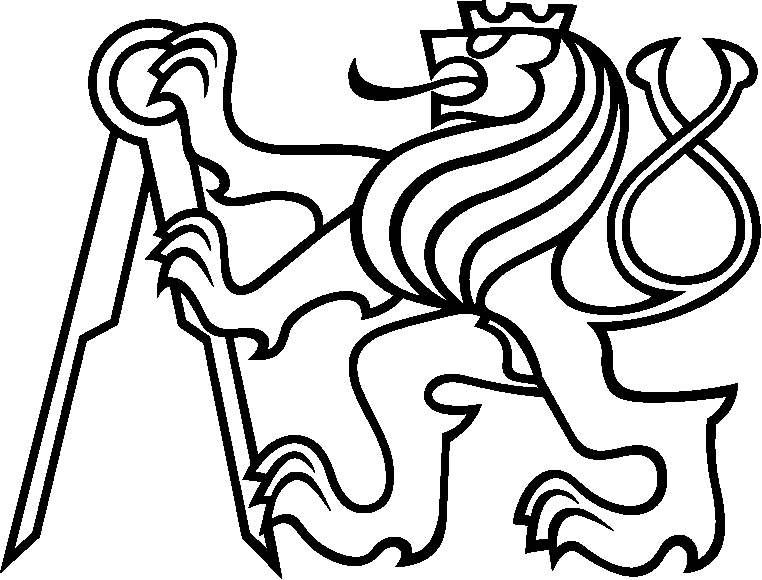
\includegraphics[width=3cm]{logo_cvut_cb} %~
\vfill
{\Large\velka{\napisBakalarka}}\\
{\Large\velka{\napisNazevI\\
\napisNazevII}}\\
{\large\velka{\napisNazevAjI\\
\napisNazevAjII}}
\vfill
{\large%
Vedoucí práce: \napisVedouci\\
\napisKatedra\\
\bigskip
\napisDatum\hfill\napisAutor}
\end{center}

\newpage
\definecolor{navodotisk}{RGB}{10,10,10}
\newcommand{\vlozZadani}{%
\Huge\textcolor{navodotisk}{\textsf{\textbf{ZDE VLOŽIT ORIGINÁLNÍ ZADÁNÍ}}}%
}
%%%\includepdf[picturecommand={\put(100,200){\vlozZadani}}]{zadani}
 % resi si zalomeni sam

\begin{abstract}

\bigskip

\klicslova{Klíčová slova}{GIS, GRASS}

\end{abstract}

\selectlanguage{english}
\begin{abstract}

\bigskip

\klicslova{Keywords}{GIS, GRASS}

\end{abstract}
\selectlanguage{english}


\newpage
\newcommand{\odsaditodzhora}{\hskip1pt\vfill}

\odsaditodzhora
\noindent Declaration of authorship

I declare that the work presented here is, to the best of my knowledge and
belief, original and the result of my own investigations, except as acknowledged.
Formulations and ideas taken from other sources are cited as such.

December 21, 2013

\begin{flushleft}
\begin{tabular}{cp{0.3\textwidth}c}
In Mosty u Jablunkova, 
& 
&
..................................
\\
&&
(author’s signature)
\end{tabular}

\end{flushleft}
\newpage

%%% -> ML: chybi ;-)

\odsaditodzhora
\noindent Poděkování


\newpage

\newpage
\tableofcontents


\newpage
\pagestyle{fancy}

\necislovana{Introduction}

In recent decades tremendous development of information technology has fundamentally changed many disciplines.

Photogrammetry has successfully taken advantages of this development, and nowadays 
it is using different methods and equipment, which allows to obtain and process data 
in huge scales achieving very good accuracy. Some of the currently used 
methods has been known for several decades, however technology was not so advanced to be use 
 in practice. 

Information technology has caused blurring of borders between disciplines. 
Photogrammetry has been affected by computer vision, which evolved independently until 2000's. After that it is possible 
to see growing trend of combining knowledge from both fields. 

Both photogrammetry and computer vision are dealing with information recorded in photo. Computer vision 
methods are employed in robotics, dealing with determination of robot position and retrieving structure 
of environment which surround the robot.
Photogrammetry is used to produce digital terrian models (DTM), precise structure of objects or orthophotos. 
Orthophoto is created in 
orthorectification process, which is transformation form perspective projection into orthogonal projection.
Unlike non-orthorectified pohotography the orthophotos can be merged together into seamless map. Recently 
orthophoto has been widely used by map services like Google Maps or Mapy.cz. Orthorectified photo 
has same scale in all parts, therefore it is possible to measure true distances as in map. During orthorectificaion distortion 
caused by tilt of camera (if photo is not vertical) together with elevation differences are removed.

TODO PICTURES


The core of photogrammetry is quickly moving  from  hardware towards software. In past it was necessary to have special 
expensive equipment to perform photogrammetric measurement. Nowadays, thanks to current state of the art software, 
 it is possible to use higher level digital cameras to perform precise photogrammetric measurements. 
 Currently it is even possible to process data from optically inaccurate low level cameras.
 The inaccuracy is compensated by processing big number of photos bringing redundancy, 
 which positively affects precision of retrieved information.
 
As a consequence of these changes, photogrammetry has not longer been domain of few professionals but it has 
become to be used by much wider audience. 

Geographical information system (GIS) is software which is used for storing and processing information,
with spatial component. For instance  GIS is employed on backed of map portals (e. g. Google Maps) therefore nearly 
everybody uses its products nowadays. 
The GIS systems are also used for analyzing spatial phenomenons, which
are utilized by decision makers (politicians, managers), to get in-depth knowledge about the 
phenomenon they are dealing with.

With growing importance of software there comes a question of licenses. There are two 
main branches: proprietary software and free software. Most of proprietary software is not available in 
form of source code. The license of proprietary software allows to use it under certain terms and usually user 
has to buy it. Proprietary software works like blackbox, because user has no chance to investigate the source 
code and realize what is happening. Therefore user can only believe to software provider
that software is doing what the provider advertises. 
For instance it can be problem when some data are analyzed
because the user loses control 
over the data in processing chains which uses proprietary software in some steps.
This also posses very serious security threads, because the software can do some hidden activity against user,
e. g. obtaining personal data or tracking user activity.

Despite the fact that current complexity of software is so huge,
that single human is not capable to really understand every piece of software, which uses,
free software does not posses disadvantages of proprietary softwares.
Transparency of the free software makes its source code subject to public control 
carried out by community of developers which are gathered around the project.
All popular free software projects have such a active communities, therefore it is
very unlikely that same malicious code would be included into the project.
Moreover if such a case would happen, it would not take a long time until such a change 
would be spotted.

\necislovana{Essential principle}

Both photogrammetry and computer vision are dealing with retrieving structure of scene from set of photos 
covering the scene. The methods for retrieving the structure are based on pinhole camera model, which 
describes relation of photo point to the 3D point in object camera system.
Parameters which characterizes pinhole camera model are called interior orientation parameters.
The relation is showed in this picture:
TODO

Image plane is represented by digital cameras image sensor, which  creates image converting light into electronic signal.
Then the signal is processed inside the camera giving output as photograph, which is stored in a digital format. 
Image sensor is divided into cells, which measure intensity of fallen light on their surface. The pixel value in final 
photograph is based on the measured intensity of cell or group of cells. The pixel location in image corresponds
to the location of the cells on the chip.


All light rays going from the object points and falling on image sensor are going through the same point in pinhole camera model.
The point is called projective center. The ray which is perpendicular to the image plane is called principal ray and the point 
where the principal ray intersects the image plane is called principal point. It is clear that during the projection of
3D scene onto 2D plane it must be some information lost because of dimensional reduction.


If 3D coordinates of point are known it is able to reproject it on the image plane. However as a consequence 
of the dimension reduction it is not possible to determine the 3D coordinates of the point from 2D photo coordinates, 
only the ray can be reconstructed.


However if the point is located at least on a two photos, which were taken from different positions and these positions 
 are known (this is called exterior orientation), it is possible 
to reconstruct 3D coordinates of the point, because it lies on the intersection of the photo rays.

PICTURE


In this thesis there are introduced and used such a methods leading to retrieval of the scene structure from the 
the set of photos, which is based on such a simple principle! Computer vision calls it structure from motion 
and photogrametry uses it for creation of orthophoto, DTM or structure of object.


\newpage

\section{Theoretical part}


\subsection{GRASS GIS}

GRASS (Geographic Resources Analysis Support System) GIS is open source GIS software cabable of processing raster, vector and imagery data. 
GRASS GIS can be considered one of 
the most oldest active software project. The development of GRASS GIS begun by U.S. Army CERL  laboratory
in first half of 1980s. In 1990s U.S.Army gradually ceased developing GRASS GIS. Luckily it was decided to 
release source code as public domain therefore the development could be taken over by volunteers. In the 1999 license 
of GRASS GIS was changed into GNU GPL v2. Currently GRASS GIS is developed by GRASS development 
team, which is comprised of developers spread world wide. 
 
Individual functionalities of GRASS GIS are implemented in form of small simple modules, which 
can be combined to solve complex tasks.
Unlike other GIS systems as QGIS or ArcGIS, it takes 
more time for a new users to start understand the philosophy of GRASS architecture. Developers 
has been aware of this problem, there they decided to develop graphical user interface, which 
has evolved dynamically.

Data in GRASS GIS are stored in GIS Database. GIS Database is composed of locations. Every location 
defines its projection and all data, which belongs to the location, must be reprojected to 
the projection in order to be included into the location. The location comprises from mapsets, which are used for organization 
of data into consistent units. 

Another important element of GRASS GIS is computational region. Region stores information about 
extend, which is defined by four values (north, south, east, west) of bounding box and 
two values, which defines south-north and west-east resolution. Properly set region is 
very important for raster data processing, because nearly all except import modules provides computation 
on currently set region. Vector data are processed in whole extend regardless region.

\subsection{UAV}

Unmanned aerial vehicle (UAV also known as drone) is aircraft without human pilot. Recently UAVs are ingloriously known for
their heavy military employment especially by USA in Afghanistan and Pakistan. These military drones are equipped with state of the art 
technology and their construction is similarly complex as small aircraft.  
The number of military UAVs is quickly raising and nowadays USA traines more UAV operators than fighter plane pilots. 
There is also exponentially growing sector of civil drones, which is very broad category ranging
from big military like size drones to small ones in size of few decimeters. There are several types of drones e. g. airplanes,
helicopters, multicopters, paraglides, airships, baloons and others. 
Very promising category of drones are multirotor drones (e. g. hexacopters or octocopters), because they have simple construction and 
even ordinary users are able to learn control them very quickly. Together with quickly decreasing prizes of octocopters it can be expected 
that this kind of drone will become commonly used for many civil purposes.

In photogrammetry cheap UAVs can be successfully used in mapping missions for creation of DTM and orthophoto.
Main advantage of the mission are cost savings compared to missions which is performed by manned aircraft.

\subsection{Least squares}
\label{sec:least}


In linear algebra commonly solved equation is:

\begin{equation}
\label{eq:linear_eq}
\ematr{A}\evect{X} = \evect{L} 
\end{equation} 

which can be interpreted as:
\begin{itemize}
\item \evect{L} - vector of measurements
\item \evect{X} - vector of parameters, which values are searched to solve the system
\item \ematr{A} - it is matrix of the linear cost function  coefficients,  where row represents one measurement 
		  and column represents one parameter of cost function. Linear cost function $\efunc{f_{i}(\evect{X})}$
		  represents relationship between measurements \evect{L} and searched parameters \evect{X}. 
		  Least square method calls it design matrix. 
\end{itemize}

If matrix \ematr{A} is 
non singular matrix  and vector \evect{b} is non zero vector, then there exists exactly one solution 
for vector of parameters  \evect{X} to satisfy the equation. Non singular matrix is always square matrix, 
which has both column vectors and row vectors linearly independent. 

Basically every measurement is burden with some error. The errors can be devided into these main categories:  
\begin{itemize}
\item gross error - error caused by human factor or fault of instrument. If many measurements are repeated
usually it is possible to identify measurements with this errors because they are big outliers from the other measurements, which are not affected with this 
kind of error.
\item systematic error - this error always has same effect (value) on measurement.  Usually effect of this error can be 
eliminated by choosing right measurement method, calibration of instrument or taking it into account in  mathematic model.
\item random error - this error is unavoidable because it is impossible to know perfectly all factors which has impact 
on a measurement. The random errors follows normal distribution which is represented with probability density function of this shape:

TODO picture


The normal distribution is characterized by two parameters, which are standard deviation and  mean. 
If measurements are burden only with random error the mean represents accurate value and standard deviation represents 
dispersion level of measurements. 
Theoretically  if measurements of some parameter would be repeated infinite times and the measurements would be influenced only by random errors,
accurate values could be computed as mean.
It follows that it is possible to get closer to the accurate value by repeating of measuremnts, which 
leads into solving overdetermined systems. Another important implication is that if same number of measurement is perfromed by more accurate 
instrument, the mean of measurements is closer to the accurate value than the mean of measurements perform with less precise instrument.
Measurements of different accuracies, can be combined together by weighted mean
with weight of measurement $\escal{p}_{i}$ defined as:
\begin{equation}
\label{eq:wmean}
\escal{p}_{i} = \frac{\escal{const}}{\escal{\sigma}_{i}^{2}}
\end{equation} 
where \escal{const} is arbitrary chosen number which is used for calculation of all weights 
and $\escal{\sigma_{i}}$ is standard deviation of the instrument used for the measurement.
\end{itemize}

The overdetermined systems are solved in many fields which deals with measurements, where the precision matters (e. g. 
surveying, photogrammetry etc.).
As consequence of overdetermination, the design matrix \ematr{A} becomes rectangular with more linearly independent rows than independent columns 
and therefore the solution does not exist for this linear equations system \eqref{eq:linear_eq}.
Only if the measurements would be perfect it would be possible to find such a parameters vector \evect{X}, to 
solve the system of linear equations \eqref{eq:linear_eq}. 

Due to measurements imperfection it is not possible to find such a parameters of vector \evect{X} to make difference \evect{v} between measured values and 
result of cost function using the parameters equal to zero:

\begin{equation}
\label{eq:least_v}
\evect{v} = \evect{L} - \ematr{A}\evect{X}
\end{equation} 



Hence it is needed to define different condition, which allows to find optimal solution of the 
overdetermined system.

The least square method finds such a values of parameters vector \evect{X}, which 
follows condition of minimum sum of square differences \evect{v}: 

\begin{equation}
\evect{v}^{T} \evect{v} = min
\end{equation} 

TODO picture

The minimized equation can be rewritten:

\begin{equation}
\begin{split}
\evect{v}^{T} \evect{v} &= (\evect{L} - \ematr{A}\ematr{X})^{T} (\evect{L} - \ematr{A}\ematr{X}) \\
&= \evect{L}^{T} \evect{L} - 2 \evect{L}^{T} \ematr{A} \evect{X} + \evect{X}^{T} \ematr{A}^{T} \ematr{A} \evect{X}
\label{eq:least_be_part}
\end{split}
\end{equation} 

According to calculus notation least squares method searches for global minimum if the square difference function. 
The global minimum of the function can be obtained using partial derivative of parameters in cost function.
In this case derivatives are simple because it is supposed that our cost functions are linear, therefore 
its square forms  second degree polynomial e. g. parabola in \eucl{2}, paraboloid in \eucl{3} etc., which has
only one point, where all partial derivatives are equal to zero, regardless dimension of the function. The point It is 
exactly the global minimum, which the least squares method searches for!

The partial derivative of minimized function can be written as:
 
\begin{equation}
\frac{\partial diff}{\partial \evect{X}} = -2\ematr{A}^{T} \evect{L} + -2\ematr{A}^{T}\ematr{A} \evect{X} 
\label{eq:least_part}
\end{equation} 

Giving this equation equal to zero, the global minimum can :
\begin{equation}
-2\ematr{A}^{T} \evect{L} + -2\ematr{A}^{T}\ematr{A} \evect{X} = 0 
\end{equation} 

The least square determines values of parameters vector \evect{X}, which can be expressed from previous equation:
\begin{equation}
\evect{X} = (\ematr{A}^{T} \ematr{A})^{-1} \ematr{A}^{T} \ematr{L}
\end{equation}

which is essential equation of the least squares method. The equation can be solved simply by means of linear algebra.

The equation supposes that all measurements have same weigh (accuracy). The least squares method can be extended to support weights.
Weight matrix \ematr{P} contains measurements weights on the diagonal with off-diagonal being zero elements if
the measurements are not correlated.
Weigh matrix row of individual weight determines a measurement in design matrix \ematr{A} where the weight belongs.

The equation, which is minimized by least squares is extended by weigh matrix:
\begin{equation}
\evect{v}^{T}  \ematr{P} \evect{v} = min
\end{equation}

therefore the least square equation is altered into this form:
\begin{equation}
\label{eq:least_sq}
\evect{X} = (\ematr{A}^{T} \ematr{P} \ematr{A})^{-1} \ematr{A}^{T} \ematr{P} \ematr{L}
\end{equation}

\subsubsection{Non-linear least squares}
\label{sec:non_least}
So far it was supposed that cost function is linear and thus global minimum can be found simply by means of linear algebra  \eqref{eq:least_sq}.
Unfortunately in many cases the relationship between parameters and 
measured values is not linear, hence it is needed to adapt linear least squares equations for this case.

Unlike linear least squares, which square of cost function is represented by function  (parabola, paraboloid...) with just one point where all
partial derivatives are being zero, the non-linear cost function can have many such a points (local minimas, stationary points, maximas). 

This problem of non-linearity can be solved by linearization of non-linear equations.
The main idea of linearization process is to approximate the cost function with first degree Taylor polynomial,
which is linear and therefore it is possible to use linear least square equation \eqref{eq:least_sq} 
to solve non-linear problem. 

Approximation of cost function with a first degree Taylor polynomial can be written as:
\begin{equation}
\efunc{T^{f_{i}, X_{0}}_{1}} = f_{i}(X_{0}) + \frac{\partial \efunc{f_{i}}}{\partial {X_{0}}} f_{i}'(X_{0}) (X -  X_{0}) 
... \frac{\partial \efunc{f_{i}}}{\partial {X_{0}}} f_{i}'(X_{n}) (X -  X_{0}) 
\end{equation}

where:
\begin{itemize}
\item $\evect{X}_{0}$ is point where the Taylor polynomial touches function, which it approximates. E. g. first degree Taylor polynomial 
      is line, which is tangent of function at point $X_{0}$ in \eucl{2}, in \eucl{3} it is tangent plane and n-dimensional 
      space it is tangent hyperplane.
\item \evect{X} is point where a Taylor polynomial returns approximate value of function $\efunc{f}_{i}$
\end{itemize}

TODO picture 

Least squares Taylor polynomial can be written as:

\begin{equation}
\efunc{T^{f_{i}, X_{0}}_{1}} = f_{i}(X_{0}) - a_{0} x_{0} ... a_{n} x_{k} 
\end{equation} 

in matrix form:
\begin{equation}
\efunc{T^{f_{i}, X_{0}}_{1}} = \evect{v} = \evect{L_{X_{0}}} - \ematr{A}\evect{dx}
\end{equation} 

And analogous equation to \label{eq:least_v} can be derived:
\begin{equation}
\evect{v} = \evect{L} - \efunc{T^{f_{i}, X_{0}}_{1}}
\end{equation} 
 
Taylor polynomial member can be rewritten as:
\begin{equation}
\begin{split}
\evect{v} &=  \evect{L_{X_{0}}} - \evect{L} - \ematr{A}\evect{dx} \\
          &= \evect{l} - \ematr{A}\evect{dx}
\end{split}
\end{equation}

If the differences vector is substituted into least squares minimization criteria:
\begin{equation}
\label{eq:min_cond}
\evect{v}^{T}  \ematr{P} \evect{v} = min
\end{equation}

the essential equation for non linear least squares can be derived 
following same steps as in linear least squares:

\begin{equation}
\label{eq:non_least_sq}
\evect{dx} = (\ematr{A}^{T} \ematr{P} \ematr{A})^{-1} \ematr{A}^{T} \ematr{P} \ematr{l}
\evect{X} =  {\evect{dx} -  \evect{X_{0}}}
\label{eq:least_sq}
\end{equation}

If the equation is compared to the linear least squares equation \label{eq:least_sq},
 it is slightly different. Instead of parameters vector \evect{X} there is used 
parameters vector of differences \evect{dx} and measurement vector \evect{L} is analogous to vector \evect{l}. In this two minor 
substitutions there are hidden major limitations of the non-linear least squares method, 
where the prize for approximation is paid. 

As it was already mentioned the Taylor polynomial requires some point $\evect{X_{0}}$, where it is tangent to 
approximated function.
This approximation is good in close surroundings of point $\evect{X_{0}}$, however as the distance 
grows the approximation error may increase significantly.

Therefore, unlike linear least square method, non-linear least squares requires initial 
value of parameters \evect{X}. If the initial values are not accurate 
enough, it is possible to iteratively run linear least squares subsequently using parameters vector \evect{X}
from previous iteration to eventually approach global minimum of the cost function. 
Therefore the closeness of the initial point $\evect{X_{0}}$ to global minimum affects how many iterations (speed of convergence)
are needed to achieve optimal solution (global minimum).

Unfortunately the non-linear least square method has another one even more serious pitfall, which 
does not guarantee that it will iterate towards global minimum at all!
In this case the found parameters \evect{X} are completely wrong because 
it does not satisfies minimum squares difference condition \label{eq:min_cond}. If the initial values are 
inaccurate the least squares can iterate toward other points with zero derivation as local minimas or stationary points.  
This is caused by run-off of non-linear functions, which has more points with zero derivative,
and therefore result depends on initial point given by $\evect{X_{0}}$  of non-linear least squares iteration.


\subsubsection{Least squares properties}

It was proved that above derived least square method is solution of Gauss-Markoff model, which 
says if measurements \evect{L} are random with known covariance matrix $\ematr{\Sigma}_{l}$  and vector of parameters \evect{X} is non-random, then
vector \evect{dx}  has the lowest variance and it is unbiased.If density functions of measurements are normally 
distributed then values obtained from cost functions using  computed parameters lies in maximum of the density
function. In other words posses maximum likehood.

The weight matrix is calculated form covariance matrix in similar way as weights in weighted mean \eqref{eq:wmean}:
\begin{equation}
\ematr{P} = \frac{\escal{const}}{\escal{\Sigma}_{i}^{2}}
\end{equation} 

\escal{const} is chosen arbitrary, therefore it can be selected as unit a priori weight standard deviation $\sigma_{0}$. 


Unbiased unit weight standard deviation $\hat{\sigma}_{0}$ can be also estimated a posteriori as:
\begin{equation}
\escal{\hat{\sigma}}_{0}^{2} = \frac{\evect{v}_{T} \ematr{P}  \evect{v}}{\escal{r}}
\end{equation} 

where \escal{r} is redundancy, which is difference of columns number from rows number of design matrix \ematr{A}.

Covariance of calculated parameters $\ematr{\Sigma}_{x}$ can be get from:
\begin{equation}
\ematr{\Sigma}_{\hat{x}} = \escal{\hat{\sigma}}_{0}^{2} (\ematr{A}^{T} \ematr{P} \ematr{A})^{-1}
\end{equation} 

and a posteriori covariance matrix $\ematr{\Sigma}_{\hat{l}}$ of measurements can be obtained from:
\begin{equation}
\ematr{\Sigma}_{\hat{l}} =  \ematr{A} \ematr{\Sigma}_{\hat{x}} \ematr{A}^{T}
\end{equation} 

\subsubsection{Free network least squares}
\label{sec:free_net_least}

In geodesy it can happen that columns of design matrix \ematr{A}
are not linearly independent. This can be caused by missing information
about coordinate system in the design matrix. This issue is called datum deficiency.
Datum deficiency makes normal matrix $ \ematr{A}^{T} \ematr{P} \ematr{A}$ non invertible and therefore 
least squares equation \label{eq:non_least_sq} cannot be solved.
In order to avoid the datum deficiency issue it is needed to keep some parameters fixed, 
which means that columns of the fixed parameters are excluded from design matrix\ematr{A}.

Photogrammetry deals with three dimensional spaces, which requires fixing of at least  
two points and another point with one coordinate to avoid datum deficiency problem, because
three dimensional coordinate system is defined by three coordinates of shift vector, three rotation angles and scale factor. 

If there is not enough fixed points, the network has to be adjusted as free network.
One of possible methods how to adjust free network is calculation of pseudo inverse matrix of the normal matrix instead of
inversion. Another option is adding inner constraints the design matrix.

\subsection{Short introduction to photogrammetry}

Essential information which must be obtained to retrieve product of photogrammetric is 
interior orientation and exterior orientation of camera.
Exterior and interior orientation together describes relation between object point and
it's corresponding image point in two subsequent transformations.

\subsubsection{Interior orientation}

Interior orientation describes relation between measured 2D photo coordinates 
and corresponding 3D in camera coordinate system.

Camera coordinate system has origin in projective point, z axis heading out of the scene  and x, y axes being parallel to photo plane. 

Photogrammetry equations are based on pinhole camera model, which describes projection of 3D point onto image plane:

Interior orientations parameters describing pinhole camera model are:
\begin{itemize}
  \item Focal length \escal{f} - it is distance of projective center from principal point.
  \item Principal point coordinates - In ideal case location of principal point would be exactly in the middle 
	of the photo.  However in most cases there is some shift of principal point from the photo center due to
	camera construction inaccuracies.
\end{itemize}

Camera optical system is imperfect, therefore it deviate from the ideal pinhole model which 
 causes distortion of photo.
The effect of distortion can be reduced by applying distortion corrections. Commonly 
used model for distortion correction is Browns model \cite{brown1966distortion}.
The model defines these two types of distortion:
\begin{itemize}
  \item Radial distortion - it depends on distance from principal point. Cause of the distortion is spherical shape of the 
  lens in camera optical system.
  \item Tangential distortion - it is perpendicular to direction of radial distortion. It is caused by 
       imperfect alignment of lenses in camera optical system.
\end{itemize}

Mathematically brown model is written:

\begin{equation}
\label{eq:undistort}
\begin{split}
\escal{x}^{u} =& (x^{ph} - x^{pp})(1 + K_{1}r^2 + K_2r^4 + ...) + \\
&(P_1(r^2 + 2(x^{ph} - x^{pp})^2) + 2P_2(x^{ph} - x^{pp})(y^{m} - y^{pp}))(1 + P_3r^2 + P_4r^4 ...) \\
\escal{y}^{u} =& (y^{ph} - y^{pp})(1 + K_1r^2 + K_2r^4 + ...) + \\
&(P_2(r^2 + 2(y^{ph} - y^{pp})^2) + 2P_1(x^{ph} - x^{pp})(y^{m} - y^{pp}))(1 + P_3r^2 + P_4r^4 ...) \\
r =& \sqrt{(x_{ph} - x^{pp})^2 + (y^{ph} - y^{pp})^2}
\end{split}
\end{equation}
where:
\begin{itemize}
  \item $\escal{x}^{u}$ and $\escal{y}^{u}$  are undistorted coordinates likewise corrected of the principal point shift.
  \item $\escal{x}^{ph}$ and $\escal{y}^{ph}$ are measured photo coordinates.
  \item $\escal{K}_{i}$ are radial distortion coefficients.
  \item $\escal{P}_{i}$ are tangential distortion coefficients.
\end{itemize}


The relation of photo coordinate system and undistorted coordinates is defined as:

\begin{equation}
\begin{split}
&\escal{x}^{u} = \frac{\escal{X}^{cam}}{\escal{Z}^{cam}} \\
&\escal{y}^{u} = \frac{\escal{Y}^{cam}}{\escal{Z}^{cam}}
\end{split}
\end{equation}

which is clearly visible on this picture, describing pinhole camera model:

TODO picture


\subsubsection{Exterior orientation}

After transformation of 2D photo points into 3D camera coordinate system it is needed to transform it into object coordinate space,
because usually the object coordinate system is not coincident with camera coordinae system. 
Object space coordinate system must be cartesian otherwise it must be transformed before into cartesion one before applying exquations 
derived bellow. 

Exterior orientation is defined by position of camera center in object space and orientation of camera coordinate system in the object space.
Photogrammetry uses representation of orientation by euler angles and rotation matrix.
The euler angles are group of three angles, which describes three subsequent rotations
 around axes of 3D coordinate system. 
 Order of euler angles is important, because in case of breaching it, resulting orientation is different. 
 In this work there is used notation where at first rotation around y axis by angle $\escal{\phi}$ is 
 perform, then system is rotated around x axis  by angle $\escal{\omega}$ and
 the last rotation is perform around z axis by angle $\escal{\kappa}$.
 
Mathematically the three euler rotations can be expressed as multiplication of three corresponding
rotation matrices:
 \begin{equation}
 \begin{split}
\ematr{R} &= \ematr{R}_{z}(\escal{\kappa}) \ematr{R}_{x}(\escal{\omega}) \ematr{R}_{y}(\escal{\phi}) \\
	  &= \begin{pmatrix}
	      cos(\escal{\kappa}) & sin(\escal{\kappa}) & 0 \\
	      -sin(\escal{\kappa}) & cos(\escal{\kappa}) & 0 \\
	      0 & 0 & 1
	      \end{pmatrix}
	      \begin{pmatrix}
	      1 & 0 & 0 \\
	      0 & cos(\escal{\omega}) & sin(\escal{\omega}) \\
	      0 & -sin(\escal{\omega}) & cos(\escal{\omega} 
	      \end{pmatrix}
	      \begin{pmatrix}
	      cos(\escal{\phi}) & 0 & -sin(\escal{\phi}) \\
	      0 & 1 & 0 \\
	      sin(\phi) & 0 & cos(\phi)      
	      \end{pmatrix} \\
	  &=  
	      \small
	      \begin{pmatrix}
	      cos(\escal{\kappa}) cos(\escal{\phi}) + sin(\escal{\kappa}) sin(\escal{\omega}) sin(\escal{\phi}) & 
	      sin(\escal{\kappa}) cos(\escal{\omega})  & 
	      -cos(\escal{\kappa}) sin(\escal{\phi}) + sin(\escal{\kappa}) sin(\escal{\omega}) cos(\escal{\phi}) 
	      \\
	      -sin(\escal{\kappa}) cos(\escal{\phi}) + sin(\escal{\kappa}) sin(\escal{\omega}) sin(\escal{\phi}) & 
	      cos(\escal{\kappa}) cos(\escal{\omega})  & 
	      sin(\escal{\kappa}) sin(\escal{\phi}) + cos(\escal{\kappa}) sin(\escal{\omega}) cos(\escal{\phi}) 
	      \\	      
	      cos(\escal{\omega}) sin(\escal{\phi}) & 
	      -sin(\escal{\omega})  & 
	      cos(\escal{\omega}) cos(\escal{\phi}) 
	      \\		      
	      \end{pmatrix} 
\end{split}
\end{equation}

\subsubsection{Basic formula of photogrammetry}

Merging interior and exterior orientation together direct relation between corresponding 3D point in object space and 2D point
in photo:

\begin{equation}
\label{eq:col_eqs}
\begin{split}
&\escal{x}^{u} = -\escal{f}\frac{\ematr{R}_{11}(\evect{X}^{obj} - \evect{X}^{obj}_{pc}) + 
                                  \ematr{R}_{12}(\evect{Y}^{obj} - \evect{Y}^{obj}_{pc}) + 
                                  \ematr{R}_{13}(\evect{Z}^{obj} - \evect{Z}^{obj}_{pc})                                  
                                  }{
				  \ematr{R}_{31}(\evect{X}^{obj} - \evect{X}^{obj}_{pc}) + 
                                  \ematr{R}_{32}(\evect{Y}^{obj} - \evect{Y}^{obj}_{pc}) + 
                                  \ematr{R}_{33}(\evect{Z}^{obj} - \evect{Z}^{obj}_{pc})     
                                  } \\
&\escal{y}^{u} = -\escal{f}\frac{\ematr{R}_{21}(\evect{X}^{obj} - \evect{X}^{obj}_{pc}) + 
                                  \ematr{R}_{22}(\evect{Y}^{obj} - ) + 
                                  \ematr{R}_{23}(\evect{Z}^{obj} - \evect{Z}^{obj}_{pc})                                  
                                  }{
				  \ematr{R}_{31}(\evect{X}^{obj} - \evect{X}^{obj}_{pc}) + 
                                  \ematr{R}_{32}(\evect{Y}^{obj} - \evect{Y}^{obj}_{pc}) + 
                                  \ematr{R}_{33}(\evect{Z}^{obj} - \evect{Z}^{obj}_{pc})     
                                  }
\end{split}
\end{equation}

These two equations are called collinearity equations, where
\begin{itemize}
  \item $\escal{x}^{u}$ and $\escal{y}^{u}$ are undistorted coordinates \eqref{eq:undistort}
  \item $\evect{X}^{obj}$, $\evect{Y}^{obj}$, $\evect{Z}^{obj}$ are the point coordinates in object space
  \item $\ematr{R}$ is rotation matrix describing camera system orientation
  \item $\evect{X}^{obj}_{pc}$, $\evect{Y}^{obj}_{pc}$, $\evect{Z}^{obj}_{pc}$ are coordinates of prjection center
  \item \escal{f} is focal length
\end{itemize}

TODO undistorted coords

\subsection{Short introduction into computer vision}

\subsubsection{Homogeneous coordinates}

Computer vision uses homogeneous coordinates, which allows to mathematically express some relations
 in more elegant way than using coordinates in cartesian form. 

3D point in homogeneous coordinates is defined as:

\begin{equation}
\ehvect{x} = (\escal{x}, \escal{y}, \escal{z}, \escal{w})
\end{equation}

\escal{w} component is called scale.

The transformation of homogeneous point into cartesian coordinates is done dividing 
the coordinates by scale:
\begin{equation}
\evect{x} = (\escal{x} / \escal{w}, \escal{y} / \escal{w}, \escal{z} / \escal{w})
\end{equation}

Using homogeneous coordiantes it is possible to write all cartesian points plus points in infinity.
Infinite homogeneous point is written as: 

\begin{equation}
\ehvect{x} = (\escal{x}, \escal{y}, \escal{z}, \escal{0})
\end{equation}

which is impossible to express using cartesion coordiantes with finite numbers:

\begin{equation}
\evect{x} = (\escal{x} / \escal{0}, \escal{y} / \escal{0}, \escal{z} / \escal{0})
\end{equation}

TODO graphic interpretation of hom coords 

Picture shows 


Thanks to homogeneous coordinates for planes in \eucl{3} and lines in \eucl{2} it allows to 
use simple vector linear algebra operations 
to get useful information.

Plane in \eucl{3} can be written as:

\begin{equation}
\escal{a}\escal{x} + \escal{b}\escal{y} + \escal{c}\escal{z} + \escal{d} = 0
\end{equation}

Using homogeneous coordinates it can be expressed as vector:

\begin{equation}
\ehvect{\pi} =  (\escal{a}, \escal{b}, \escal{c}, \escal{d})
\end{equation}


Line in \eucl{2} is defined by equation:
\begin{equation}
\escal{a}\escal{x} + \escal{b}\escal{y} + \escal{c} = 0
\end{equation}

Using homogeneous coordinates it can be also written as vector:

\begin{equation}
\ehvect{l} =  (\escal{a}, \escal{b}, \escal{c})
\end{equation}

It is easy to find out whether point lies on line in \eucl{2}:

\begin{equation}
\ehvect{x}^{T} \ehvect{l} = 0
\end{equation}

or whether if a point lies on plane:
\begin{equation}
\ehvect{x}^{T} \ehvect{\pi} = 0
\end{equation}


In \eucl{3}, line cannot be written so elegantly.
One of options is to define it given points $\ehvect{p}$ and $\ehvect{q}$ as:
\begin{equation}
 \ehvect{l} = \escal{\mu}\ehvect{q} + \escal{\lambda}\ehvect{p}
\end{equation}

If the point is given as direction of the line $\ehvect{d} = (x, y, z, 0)$ (it is point in infinity), the equation get simplified to:
\begin{equation}
\ehvect{l} = \ehvect{d} + \escal{\lambda}\ehvect{p} \label{eq:hline}
\end{equation}
TODO where not zeros

Computation of lines intersection ($\ehvect{l}, \ehvect{l}'$) can be done also in very simple way by cross product in \eucl{2}:

\begin{equation}
\ehvect{x} = \ehvect{l} \times \ehvect{l}' \label{eq:def_hline_pts}
\end{equation}

Note that with homogeneous coordinates it is possible to express intersection of parallel lines, which lies at infinity, 
therefore it's scale is equal to 0.

TODO dualism

Similarly line can be derived as cross product of two points:

\begin{equation}
\ehvect{l} = \ehvect{x} \times \ehvect{x}'
\end{equation}


\subsubsection{Basic formula of computer vision}

Computer vision uses this equation to describe relationship between
object space and image space:

\begin{equation}
\begin{pmatrix}
   \escal{x} \\
   \escal{y} \\
   \escal{1} \\
\end{pmatrix}
=
\begin{pmatrix}
   & \escal{f_{x}} & 0     & \escal{c_{x}}\\
   & 0     & \escal{f_{x}} & \escal{c_{x}}\\
   & 0     & 0     & 1\\
\end{pmatrix}
\begin{pmatrix}
&\ematr{R}&\evect{t}\\
\end{pmatrix}
\begin{pmatrix}
   \escal{X} \\
   \escal{Y} \\
   \escal{Z} \\
   \escal{1} \\
\end{pmatrix}
\end{equation}

In essence the equation is equivalent to collinearity equations \eqref{eq:col_eqs} which are used in photogrammetry.
The two models differs only in definition of camera coordinate system.
Computer vision uses left handed system with z axis heading into 
the scene. Unlike  Photogrammetric system defines z axis in the opposite direction heading out of the scene, thus 
it is right handed. Otherwise the basic formula embodies exactly same transformations as 
collinearity equations written in different way.

The equation can be abbreviated as:

\begin{equation}
\label{eq:p_exp}
\escal{w} \ehvect{x} = \ematr{K} \ematr{[}\ematr{R}|\evect{t}\ematr{]} \ehvect{X}
\end{equation}

TODO picture of system

where:

\begin{itemize}
\item \ematr{K} is calibration matrix which contains interior orientation parameters.  
\item \ematr{[\ematr{R}|\evect{t}]} matrix contains rotation matrix\ematr{R} and translation vector $\evect{t}$, 
	      which transforms point from object coordinate system 
	      into camera coordinate system. The camera system is left handed cartesian system originating in projective center 
	      with z axis perpendicular to image plane heading into the scene direction.
	      If the object space is right handed the rotation contains also switch of handedness,
	      which is called reflection. If the rotation matrix includes reflection its determinant is negative.
	      It must be taken into account before 
	      The translation vector $\evect{t}$ can  be transformed in object space coordiantes system:
	      \begin{equation}
	      \ehvect{C} = \ematr{R}_{T}\evect{t}
	      \end{equation}
	      giving coordinates of camera projective center. The rotation matrix \ematr{R} and projective 
	      center object coordinates $\evect{C}$
	      represents exterior orientation of camera.   
\item $\ehvect{X}$ euclidean object space coordinates extended into homogeneous form
\item $\ehvect{x}$ photo space homogeneous coordinates extended into homogeneous form
\end{itemize}

Whole projection can be merged into single matrix \ematr{P}, which is called camera matrix:

\begin{equation}
\label{eq:p_abbr}
\ehvect{x} = \ematr{P} \ehvect{X}
\end{equation}

Camera matrix \ematr{P} defines reprojection up to scale $\escal{\lambda}$, hence every camera matrix multiplied by scale gives same image points:

\begin{equation}
\ehvect{x}=\lambda\ehvect{P}\ehvect{X}
 \end{equation}

It can be interpreted as representation of ray going from the projective center. 
The object point can be located everywhere on this ray, getting always 
same image point coordinates.

\subsubsection{Two view geometry}

In this chapter, there is introduced theory, which describes mutual relation of two images. 
The core of the theory lies in epipolar geometry.

TODO picture of epipolar geometry
If same object point is identified on two images then there exists epipolar plane.
The epipolar plane contais:

\begin{itemize}
\item two rays which connects object point, with image points and camera centers of both images
\item baseline, which connects projection centers of images
\item epipoles, which are defined as intersection of image planes with baseline
\item epipolar lines, which goes through epipoles and image points. It belongs into image plane, 
      because both these points are inside this plane.  
\end{itemize}


The other relations which comes form epipolar geomatry are:

\begin{itemize}
\item All epipolar lines in image intersects in epipole. If two images are only translated along the baseline 
     the epipole is in infinity.
\item Every image point forms epipolar line in the other image. It allows to reduce space of possible occurrence of the point 
      from \eucl{2}, \eucl{1} of epipolar line, without any other information about the point e. g. object space coordinates. 
\end{itemize}

Algebraic derivation will be done beginning with description of ray in camera coordinate system.
The ray can be defined by two points.
One of them can be projection center $\ehvect{C}$, and 
image point $\ehvect{x}$ transform into camera coordinate system using pseudo inverse matrix $\ematr{P}^{+}$, 
where $\ematr{P}\ematr{P}^{+} = \ematr{I}$. After the transformation of x, direciton vector of ray is get.
Using equation \eqref{eq:hline}, it is possible to express ray as:

\begin{equation}
\ematr{X}(\escal{\lambda}) = \ematr{P}^{+}\ehvect{x} + \escal{\lambda}\ehvect{C}
\end{equation}

In second camera with camera matrix \ematr{P'} image point coordinates are:

\begin{equation}
\ehvect{x'} =  \ematr{P'}\ematr{P}\ehvect{x}
\end{equation}

and projective center of first camera is projected into epipole: 

\begin{equation}
\ehvect{e'} =  \ematr{P'}\ehvect{C}
\end{equation}

Having two points in image coordinate system of second camera it is possible to define epipolar line using \eqref{eq:def_hline_pts} as:

\begin{equation}
\ehvect{l'_{e}} =  \ehvect{e'} \times \ehvect{x'} = \ematr{P'}\ehvect{C} \times \ematr{P'}\ematr{P}\ehvect{x}
\end{equation}

Cross product of two vectors \evect{a} and \evect{b} can be also written as multiplication of matrix and vector:

\begin{equation}
\evect{a}  \times \evect{b}  = 
\begin{pmatrix}
   & 0      & \escal{a_{3}}   & \escal{a_{2}}\\
   & \escal{a_{3}}  & 0               & \escal{-a_{1}}\\
   & \escal{-a_{2}} & \escal{a_{1}}   & 0\\
\end{pmatrix}
\evect{b} = [a]_{\times} b
\end{equation}

Using this formulation of cross product thre:
\begin{equation}
\ehvect{l'_{e}}  = [e']_{\times} \ematr{P'}\ematr{P}\ehvect{x}
\end{equation}

It is evident from this equation, that matrix, which transforms photo points in the first photo into 
epipolar lines of the other photo and thus denoting relation of two images is defined as:

\begin{equation}
\ematr{F}  = [\ehvect{e}']_{\times} \ematr{P'}\ematr{P}
\end{equation}

Matrix \ematr{F} is called fundamental matrix. 

Decomposing fundamental matrix using camera matrix expansion from \eqref{eq:p_abbr}
it allows to derive another important of two view geometry, which is called essential matrix \ematr{E}.

Lets suppose that firs camera matrices are defined in this way:
\begin{equation}
\label{eq:rel_or_cam1}
\ematr{P}  = \ematr{K} \ematr{[}I|0\ematr{]}
\end{equation}
It means that first camera coordinate system coincides with object space coordinate 
system.

It's pseudo inverse matrix is:
\begin{equation}
\ematr{P}_{+} =
\begin{pmatrix}
   \ematr{K}^{-1} \\
   \evect{0^{T}} \\
\end{pmatrix}
\end{equation}

And homogeneous projection center coordinates are:
\begin{equation}
\ehvect{C} =
\begin{pmatrix}
   \evect{0} \\
    1 \\
\end{pmatrix}
\end{equation}


The second camera matrix is defined in this way:
\begin{equation}
\label{eq:rel_or_cam2}
\ematr{P}'  = \ematr{K} \ematr{[}\ematr{R}|\evect{t}\ematr{]}
\end{equation}

This relationship of two cameras is also called relative orientation, because rotation matrix \ematr{R} and vector \evect{t}
denotes position and orientation of the second camera to the first one. In order to express cameras exterior orientations in world coordinate 
system or merge it with another relative orientations it is needed to perform further transformations of the relative 
exterior orientations, see \ref{sec:ess_chain} and \ref{sec:helmert}.

Taking into account the relative orientation the equation can be simplified rewritten as:
\begin{equation}
\label{eg:funeq}
\begin{split}
\ematr{F}  &= [\ematr{P}'\ehvect{C}]_{\times} \ematr{P}'\ematr{P} 
= [\ematr{K}' [\ematr{R}|\evect{t}]
\begin{pmatrix}
   \evect{0} \\
    1 \\
\end{pmatrix}]
_{\times} 
\ematr{K}' [\ematr{R}|\evect{t}]  
\begin{pmatrix}
   \evect{K}^{-1} \\
   \evect{0}^{T} \\
\end{pmatrix} \\
&= [\ematr{K}' \evect{t}]_{\times} \ematr{K}'\ematr{R}\ematr{K}^{-1} 
\end{split}
\end{equation}

Now comes little bit more difficult part.
This formula,
which applies for any non-singular matrix \ematr{K} and vector \evect{t}:
\begin{equation}
[\evect{t}]_{\times} \ematr{K} = \ematr{K}^{-T}[\ematr{K}^{-1}\evect{t}]_{\times}
\end{equation}

If the formula is applied to \eqref{eg:funeq}:  
\begin{equation}
\begin{split}
\ematr{F}  &= [\ematr{K}' \evect{t}]_{\times} \ematr{K}' \ematr{R} \ematr{K}^{-1} \\
	   &= \ematr{K}^{-T} [\ematr{K}'_{-1} \ematr{K}' \evect{t}]_{\times} \ematr{R} \ematr{K}^{-1} \\
	   &= \ematr{K}^{-T} [\evect{t}]_{\times} \ematr{R} \ematr{K}^{-1}
\end{split}
\end{equation}

This equation reveals very important fact about fundamental matrix, which says that the transformation performed 
by fundamental matrix can be divided into three main steps.
At first photo point of first image is transformed into the first camera coordinate system. Result of the transformation is 
point in the infinity, which describes ray represented by image point. 
After that the ray is projected into second camera coordinate system. This is done by so called essential matrix:
\begin{equation}
	 \ematr{E}  = [\evect{t}]_{\times} \ematr{R}
\end{equation}


As the last step, the ray is projected into the second image as epipolar line.


It implies that with known exterior orientation it is possible to define essential matrix. 
Morover if interior orientation of cameras of both photos are known it is possible to determine fundamental matrix,
which describes relation of a two photos.

\subsubsection{Triangulation of points}
\label{eq:triang}

If the measurements would be precise, the 3D point 
would lie in intersection of two rays which are lines connecting projection centers and image points 
in the photos. Unfortunately the rays are never determined so precisly, thus it is needed to deal 
 with the errors by triangulatin methods. 

One of options is linear least square method based 
on mineralization of collinearity equation \eqref{eq:col_eqs}.

The linearized collinearity can be written as:  
\begin{equation}
\label{eq:col_eqs}
\begin{split}
&\escal{x}^{un} = \frac{\escal{a}_{1}(\evect{X}^{obj}) + 
                                  \escal{a}_{2}(\evect{Y}^{obj}) + 
                                  \escal{a}_{3}(\evect{Z}^{obj}) +
                                  \escal{a}_{4}
                                  }{
				  \escal{a}_{9}(\evect{X}^{obj}) + 
                                  \escal{a}_{10}(\evect{Y}^{obj}) + 
                                  \escal{a}_{11}(\evect{Z}^{obj}) +
                                   1  
                                  } \\
&\escal{y}^{un} = \frac{\escal{a}_{5}(\evect{X}^{obj}) + 
                                  \escal{a}_{6}(\evect{Y}^{obj}) + 
                                  \escal{a}_{7}(\evect{Z}^{obj}) +                                 
                                  \escal{a}_{8}
                                  }{
				  \escal{a}_{9}(\evect{X}^{obj}) + 
                                  \escal{a}_{10}(\evect{Y}^{obj}) + 
                                  \escal{a}_{11}(\evect{Z}^{obj}) +    
                                  1
                                  }
\end{split}
\end{equation}
 
This method is called direct linear transformation (DLT). It is easy to implement and 
there is no need to know approximate vaules. 

Main drawback of this method is that DLT model does not respects pinhole camera model, thus
the computed parametrs 

The more complicated method from computer vision is called the optimal solution. 
It is based on enforcing epipolar constraint, whith cost function 
minimizing distance of projected points from the other images to epipolar lines.

The cost function is not linear however it's derivative leads into 6 degree polynomial thus 
having 6 roots.

This method is seen by computer vision community is most accurate \cite[p. 315]{Hartley2004}.  

\subsubsection{Retrieving of exterior orientation from essential matrix}
\label{sec:ess_eo}


Rotation [\ematr{R}] and vector \evect{-t} can be retrieved from essential matrix using 
singular values decomposition (SVD):

\begin{equation}
\begin{split}
\ematr{W} &=
\begin{pmatrix}
& 0 & -1 & 0 \\
& 1 & 0 & 0 \\
& 0 & 0 & 1\\
\end{pmatrix}] \\
+- \ematr{R} &= \ematr{U}  \ematr{W} \ematr{V}^{T}\\
+- \evect{t} &= \evect{U}_{3,:}
\end{split}
\end{equation}

where matrices \ematr{U} and \ematr{V} are two rotation matrices  obtained for SVD decomposition.
The retrieved ration \ematr{R} matrix and the shift vector \evect{t} are defined up to sign,
which causes four ambiguity. 

The four possible exterior orientation, which gives for possible solutions, are:

\begin{equation}
[\ematr{R}|\evect{t}],
[\ematr{R}|\evect{-t}],
[\ematr{-R}|\evect{t}],
[\ematr{-R}|\evect{-t}],
\end{equation}


The ambiguity of signs can be solved by assumption that all object points has to be in front
of both photo planes:




\subsubsection{Merging of relative orientations}
\label{sec:ess_chain}

If two relative orientations are merged together, as first step, it is necessary to calculate scale of the two relative orientations.
The scale can be calculated from corresponding distances in both coordinate system. 
It can be used distances of 
object points and object coordinates of projective center of camera, which are present in both relative orientations.

The scale can be computed by this equation:
\begin{equation}
\escal{s}_{ro2-1} = \frac{\mathbf{\evect{X}^{ro1}_{1} - \evect{C^{ro1}_{1}}}}
	                {\mathbf{\evect{X}^{ro2}_{1} - \evect{C^{ro2}_{1}}}}
\end{equation}

where ro1 denotes destination orientation of transformation and ro2 is the transformed relative orientation. 

The equation gets simplified if the relative orientation coordinate system  corresponds to the shared camera system: 
\begin{equation}
\escal{s}^{ro2-1} = \frac{\mathbf(\evect{X}_{ro1})}
	                 {\mathbf(\evect{X}_{ro2})}
\end{equation}

After the scale was determined it is possible to transform exterior orientation in relative system of photo pair into the common relative system.
In order to be transformation easy to express, the common relative system is defined by arbitrary relative orientation of pair and other 
relative orientations are subsequently transformed into this system. 

Set of photos, which can be transformed into common coordinate system, is composed of the relative orientations
which comprise connected component of undirected graph where nodes denotes photos and edges represents relative orientations. 
In other words it is possible to transform relative orientation into the common relative coordinate system only if there 
exist continuous chain of relative orientations where every two neighborhood relative orientations in the chain shares one photo.

TODO PICTURE

The transformation of relative orientations from 1 to n, with common system defined by 1 can be written as: 
\begin{equation}
\label{eq:comm_rel}
\begin{split}
&\ematr{P}_{1} = [\ematr{I}|\evect{O}] \\
&\ematr{P}_{2} = [\ematr{R}^{ro1}|\evect{t}_{ro1}] \\
&\ematr{P}_{3} = [\ematr{R}^{ro1} \ematr{R}^{ro2}| \ematr{R}^{ro1} \evect{t}^{ro2} \escal{s}^{ro2-1}] \\
&\ematr{P}_{n} = [\ematr{R}^{ron} \ematr{R}^{ro(n - 1)}| R^{ro(n - 1)} \evect{t^{ron}} {s}^{ron- (n-1)}] \\
\end{split}
\end{equation}


This equation works for chain of relative orientation, where the shared camera in first relative orientation has 
projection matrix defined by $[\ematr{R}|\evect{t}]$ matrix and the merging second relative orientation is 
defined $[\ematr{I}|\ematr{O}]$. If the camera is defined be the switched coordinate systems, it is needed to 
transform system by multiplication of rotation by $\ematr{R}^[T]$ and shift by $-\ematr{R}^[T]$.

\subsubsection{Helmert transformation}
\label{sec:helmert}

Helmert transformation equation can be written as:
\begin{equation}
\ematr{X}_{t} = \evect{t} + \escal{s}\ematr{R}\evect{X}] \\
\end{equation}
where \ematr{R} is rotation matrix, \escal{s} is scale scalar and  \evect{t} is translation vector.
The transformation is defined by seven parameters (three translation coordinates, three rotation angles angles and scale).
In order to get these parameters which defines relation of two coordinate system it is needed to know at least two corresponding points and  another one with 
at least one known coordinate in both systems. 



\subsection{Bundle block adjustment}

Bundle block adjustment is method (BBA), which uses the least square technique (\ref{sec:least}) to refine scene parameters. 

The main advantage of bundle block adjustment method is that the method takes into account whole scene and therefore it utilizes 
maximum information for adjustment of scene parameters, which leads to more accurate results.
The principle of BBA has been known for very long time since 1950s,
however the method has been employed in practical applications since 1990's, because the performance of computers had not been 
sufficient enough before. 

Cost functions of BBA least squares method are photogrammetric collinearity equations \label{eq:col_eqs}.

Unfortunately collinearity equations are non linear, hence the non-linear least square method \ref{sec:non_least} must be used therefore 
it is needed to provide sufficiently accurate initial values for finding values of parameters in global minimum of cost function.

Thanks to the least squares method BBA is very flexible in terms of choosing of parameters to be adjusted. 
It is possible to select various combinations of interior, exterior orientations and object points coordinates parameters 
and refine them using BBA. 


The BBA method is described on practical this practical example.
There are three photos of a scene.
There were identified 3 tie points an 2 ground control points in all three photos.
Other two tie points one ground control point were identified on two photos and one ground control point and one tie point was identified 
on only one photo. 

Let say that initial values of tie points are known, but needed to be refined to improve its accuracy.
Coordinates of ground control points are known with high accuracy, therefore they do not have to be adjusted. 

Every tie point identified on image needs to refine three parameters (object coordinates). 
If the tie point is identified on a photo it yields two measurements (two collinearity equations), 
therefore it is needed to identify the tie point at least on two photos to get more measurements 
than unknowns. This makes perfectly sense because it is not possible to determine object point coordinates from one photo,
because it can lie wherever on the ray  which goes through photo plane, projection center and the object point.


Unlike tie points, ground control point does not bring any new adjusted parameters, thus
it is possible to use gcp which are identified only in one image. In this case the object coordinates 
are known, thus there is no point ambiguity on the ray as in tie point. 

In the example there are 3*3 adjusted parameters and 3 * 3 * 2 measurements for every tie point,  
1 * 3 * 3 measurements for every gcp identified, which are visible in all three photos. 
Moreover there are 2 * 3 adjusted parameters and 2 * 2 * 2 measurements for every tie point,  
1 * 2 * 3 measurements for the gcp visible in two photos.

Tie point which is identified only in one photo can not be used because number of measurements is smaller (2) than number of adjusted parameters (3).
The ground control point gives two measurements and know adjusted parameters therefore it can be included.

Overall score is 15 adjusted parameters and 43 measured parameters.

Thanks to 28 redundant measurements exterior orientation of images can be also adjusted, which adds 3 (photos) * 6 (eo params)
and also it is possible to add some of the interior parameters into adjustment, because of 10 left over redundant measurement.  
On the other hand the redundancy of measurement improves accuracy of results, which is the main point of the least square method,
therefore it should be avoided to have nearly same number of measurements and adjusted parameters.

\subsection{Orthorectification}

The orthorectificaion is process which transforms photo from perspective projection into orthogonal projection. 
\label{sec:single_ortho}
There are two main methods for producing of orthophoto. The first method is able to produce orthophoto 
from single photo if it's exterior and interior orientations are known and other information which describes
relief must be also known. This information is usually provided in form of digital terrain model (DTM), which 
can be provided in raster or vector form. Raster DTM describes relief with same density defined by resolution of the raster.
Vector DTM is comprised by continuous surface made of triangular irregular network (TIN). 
At the beginning of the orthorectificaiton empty raster is allocated, which represents orthophoto, 
covering intersection of photo scene and area of the DTM. Then coordinates are reprojected using collinearity
equations into photo coordiantes. Because the DTM surface continuous, it is needed to define 
a step which defines shift of points which are reprojected, The points can be choosen e. g. from every pixel center
of the alocated orthophoto pixel. Results of reprojection are not pixels cordinates which is integer number but 
floating points numbers. Therfore value of pixel in orthophoto can be computed by different interpolation methods,
which can take into account various number of neighborhood pixels and functions.

The other method is being used either in computer vision and photogrammetry.
Computer vision calls it structure from motion. As the method name suggests, it is primarily used for retrieving
structure of the scene, which is equivalent to creation of DTM in photogrammetry. In follows main advantage 
of the method that DTM is not needed unlike the first orthorectificaiton method. Moreover 
the DTM can be another output of the method besides the orthophoto.  The other approach requires to have at least
two photos of known exterior and interior orientation. In contrast to the first method the exterior orientaiton
can be defined in arbitrary coordinate system, because there is not needed to define relationship to DTM, 
therfore it is possble to generate orthophoto and DTM without any GCP. However 
if the results should be transformed into world coordiante system at least three GCP needs to be known
to perform helmert transformation. 


The principle of the method is based of forward ray intersection, where collinearity equations are employed..
In order to find object coordiantes
of point, it has to be identified at least on two photos, than two rays connecting projection 
center and image points are formed. The approximate object coordiantes can be find by trianglulation 
method \ref{sec:triang} and than refined by BBA, which is also in principle based on the rays 
resection.
 

\section{Analytical part}

Methods of the processing chain which are mentioned in this chapter are described in 
previous theoretical chapter.

\subsection{General solution of UAV bundle block adjustment}


In 1990s Global Positioning System (GPS) become first globally operational satellite navigation.
GPS allows 
to locate position of GPS unit with accuracy ranging  from  millimeters to decimeters depending 
on used technique and other conditions. 
GPS greatly simplified obtaining of initial values of exterior orientation with better accuracy in photogrammetric aerial mapping missions.
GPS unit together with 
inertial measurement unit (IMU), which measures its orientations in object space,
provides all needed parameters of exterior orientation. In order to be information useful it is need to determine 
leverage arm offset, which describes shift of GPS unit to the perspective center and bore-sight offset
which describes orientation of camera coordinate system towards IMU coordinate system. These two
quantities are determined in calibration process. The measured values from these two units has to
be corrected by the two quantities to represent true exterior orientation of camera coordinate system. The corrected values 
can be refined by BBA. Collinearity equations can be extended to include these corrections in order to be adjusted parameters 
 in BBA.

Before GPS was introduced, aerial photogrammetry made some a priori assumptions about the camera position,
which simplified the collinearity equation in order to get initial values of exterior orientation. 
For instance it can be assumed that the aerial photo is vertical if orientation deviates from true vertical
direction up to 2-3 degrees. Using this assumption collinearity equations can be linearized and 
approximate values can be computed easily from gcps.

Photogrammetric aerial mapping missions are prepared and carried out by experts using 
professional equipment which is properly calibrated.
As a consequence budget of such a missions
is high. These facts prevents further spreading of rigorous aerial photogrammetry methods.

Nowadays nearly everybody has camera in his pocket, thus there is big demand 
to provide solution which is very simple from the user point of view because 
vast majority of users has limited or no knowledge of photogrammetry or computer vision. 
Together with spread of UAV, the mapping missions can be performed with much lower 
cost compared to rigorous aerial photogrametry mission, which used to employ manned aircraft.

It follows the main requirement 
on solution, which needs to be simple and cheap enough,
in order to be adopted by
ordinary users, who do not want 
to spend money for other devices or spend time studying complicated methods. 
The users just 
want to take a group of photos of the scene and get the job done by the software.
The final solution should be flexible to process both terrestrial and aerial photos,
which can give both orhophoto and structure / DTM as output. There should 
not be any constraint on camera orientation because it should be able 
to process photos acquired from camera held by hand or mounted on UAV.
Because of instability of  UAVs flight track and human hand, the photos 
must be considered as oblique thus it is not possible to impose any constraints on camera orientation. 

In order to make this requirement of simplicity more specific, user should just need  
 camera to obtain structure of the scene. 
 In order to be orthophoto generated 
user would also need to employ UAV in order to get images from approximately vertical point of view.
No other hardware device should be needed. 
All other steps should be done 
using open source software which can everybody freely download and use. 

Also the solution should be flexible enough to process additional data, which may be known about a scene, 
as GCPs, positions of cameras etc. The additional data can
 increase accuracy of results and computational time  
 decreasing number of  BBA iterations needed for finding global minimum. This is very important 
 for professional photogrammetric measurements, where accuracy is very important.

As consequence of these constraints, the minimum required input can be just photos
of the scene and other information, which can be derived from photos of specific scene.

The another important requirement is to make the process as much automatic as possible, because 
if it would require a lot of time of user to go through the processing chain nobody would use it.


This processing chain should fulfill above mentioned requirements for the solution:

\begin{itemize}
\item Camera calibration - determination of camera interior orientation. There exists simple techniques for calibration
of camera based on processing of 2D patterns photos. Whole process is very simple from the user point of view, it is needed 
to print the pattern on sheet of paper, take photos of the pattern from different positions. The calibration 
is done automatically based on the photos. No other input except the photos of pattern is needed from user.
\item Tie point identification - it can be also done automatically be pattern match algorithms.
\item Retrieval of initial values for BBA - it is fully automatic process without need of any manual user input.
As input it needs tie points and interior orientation of camera, which are given by previous two steps.
\item Bundle block adjustment - fully automatic, it uses information from all three previous steps.
\end{itemize}

 
\subsubsection{Camera calibration}

Camera calibration is process, which deals with determination of interior orientation parameters including distortion.
There exists many different methods of camera calibration.

One family of calibration methods are based on photos acquiring calibration object.
The calibration object includes calibration points, which relative position to each other is  precisely determined.  

The methods can be further divided according to dimension of the object:
\begin{itemize}
\item 3D reference object based calibration - This method allows to reach very good accuracy of determined 
interior orientation parameters. One of common calibration objects is comprised of three or two
perpendicular planes, which are covered by calibration points. Drawback of 3D calibration 
is that accurate construction of the calibration object is complicated.
\item 2D plane based calibration - This calibration method is less accurate compared to 3D calibration. 
The accuracy can be improved by acquiring more photos of the calibration object.
On the other hand it is possible to use as calibration object the sheet of paper, which is much 
easier than construction of 3D calibration object.
\end{itemize}


Another method is self-calibration, which uses BBA to find values of the interior orientation parameters.
However at least initial values of focal length and principal point must be known.
Usually focal length and chip size are publicly available by manufacturer. The principal point 
can be computed dividing chip size by two, because it is supposed that it lies close to 
the middle of the photo.
It is more convenient to use 
pixels as expression, therefore focal length and principal point coordinates can be 
converted from millimeters units into pixels using photo resolution. 
The interior orientation from manufacturer information should not be interpreted as very accurate, therefore 
it has  to be made more accurate by camera calibration.
Including interior orientation as parameters of BBA
can lead into over-parametrization which can may result in inaccurate results.
In case of self-calibration it is recommended to take acquire convergent photos from many different directions and position in order
to avoid correlation of adjusted parameters. 

In order to keep interior orientation parameters stable the camera during should have fixed same zoom level,
because interior orientation parameters are very sensitive  to zoom changes \cite{labe2004geometric}.
Influence of focus is  much smaller then zoom influence and it has affect only in short distances of camera
from to scene.
Also change of the resolution may cause changes of interior orientation parameters, which mostly depends 
on specific camera type. 
Change of other camera features as exposure time or aperture does not have so significant effect on interior
orientation.

\subsubsection{Tie points identification}

The simplest way from developer point of view is to force user to identify tie points on 
the photographs manually. However users would have to waste a lot of time on such a 
dull task. Fortunately there  exist algorithms, which are able to identify tie points on photos
automatically. The state of the art algorithms are SIFT \cite{wiki:SIFT} and SURF \cite{wiki:SURF}.
These algorithms allows to identify tie points on photos, which covers same scene, without need to include any other information.
Unfortunately both algorithms are patented in USA, therefore their use should be avoided open source community.

Recently new BRISK \cite{leutenegger2011brisk} and FREAK \cite{alahi2012freak} algorithms
has been developed, which does not have patent restriction. 

Another problem of tie points matching is determination of corresponding photos, which scenes are overlapping. 
If photos are taken in strip, it is easy, because the corresponding photos are comprised form neighborhood phots 
in the chain.

If there is no apriori information about photo order, the easiest way is to use brute force and 
try to find tie points in all images in set.
However it become unsolvable problem with higher number images, because 
computational time very big. In order to avoid this, visibility map \cite{barazzetti2010extraction} can be build up. 
The visibility map is graph with photos as nodes. The graph edges connects photos and represents existing scene overlap 
in photos.  It is possible to use information from GPS and IMU units for creation of visibility map.

Another speed up can be done decreasing resolution of photos 
for first search of tie points. First search of photos only identifies correspondent photos.
In second step tie points extraction is done on full resolution but only with correspondent photos,
which were identified in the first search.

\subsubsection{Retrieving initial values for bundle block adjustment}

The next step is to utilize all known information (interior orientation and extracted 
image coordinates of tie points) to get missing initial values of parameters for BBA. 

Because collinearity equations \ref{eq:col_eqs} are the cost functions of BBA,
extracted image coordinates represents measurement,
the parameters of interior orienation are known from the input, thus only information, 
which is missing, are parameters of exterior orientation and object coordinates of 
tie points. 

There exist many methods how to obtain initial values of exterior orientations. The methods 
differ in information which they require for input, computation time and accuracy. 
In order to fulfill the set up requirements a chosen method should be able to retrieve exterior orientation 
using just image coordinates of tie points and interior orientation of camera. The method 
should be general in order to be able to process oblique photos.

There exists family of closed form computer vision algorithms,
which are able to determine relative orientation (essential matrix) from image coordinates 
of the tie points. The algorithms are based on epipolar geometry using essential matrix 
constraints to find the solution. 

The closed form algorithms are called 
according to required number of identified tie points in two pictures.
There exist eight, seven, six and five point algorithms. The five point algorithm seems to perform best in most
of cases \cite{stewenius2006recent} and it is not sensitive on planar points configuration.

Only case when the five point algorithm \cite{nister2004efficient} underperforms 
\cite{bruckner2008experimental} the others is forward motion of camera.
However this should occur in very rare cases, and it is possible 
to combine it with eight point algorithm to achieve higher accuracy.

Main disadvantage of the five point algorithm is that it can produce up to ten solution.
Hence it is needed to asses the solutions and select the correct one. The number of solutions
can be reduced by assumption that all tie points lies in front of both photo 
planes. After sorting out obviously non sense solution,
 the correct solution can be selecting the one which has minimum sum of epipolar distances, which is tie point distances
 from epipolar lines, which were computed by transforming corresponding tie points from the other photo
 using essential matrix of the solution and calibration matrix of the photos cameras.  

 TODO epipolar distance
 
Because matching algorithms are not perfect, thus  certain number of the tie points are matched 
incorrectly, hence it is needed to be the relative orientation robust enough to
deal with these outliers.

The RANSAC \cite{RANSAC} method is commonly used with this family of epipolar algorithms to 
make it more robust for effect of outliers.
Principle of RANSAC is to find such  a solution in group of measurements with outliers, 
which well approximates inliers.  

In case of the epipolar algorithms family RANSAC selects random tie points in every iteration.
The number of selected tie points is chosen according to minumum number, which the epipolar algorithm requires.
The the epipolar algorithm is launched with the selected points as input. 
Quality of returned essential matrix by epipolar algorithm is assessed by 
computing epipolar distances of tie points. There is specified some threshold of the distance which is used 
for decision whether the measurement is inlier or outlier. The other threshold, which has to be specified 
is minimum percentage of inliers from all tested points. If percentage of inliers is higher than in any previous iteration
and it satisfies the minimum percentage of inliers threshold, then
the essential matrix is set as the best fitting and iteration continues. The iteration terminates after 
maximum number of iterations returning the best fitting essential matrix.

TODO RANSAC PICTURE

After essential matrices are obtained, all needed information for calculation of initial object point coordiantes
is  available. The object points coordinates can be computed by triangulation methods \ref{eq:triang}.

\subsubsection{Common relative coordinate system}

All approximate values, which are needed for BBA collinearity cost functions are available. 
However it is not possible to adjust scene in one bundle, because
object coordinates of tie points and exterior orientations are denoted in  individual relative object coordinate systems
of the relative orientation photo pairs.

Therefore it is needed to transform all features in individual relative coordinate systems of photo pairs into 
an common relative coordinate system. First of all the common system has to be defined,
in order to make the transformation process simple it is defined by one of  relative orientation systems of photo pairs.

The next step is to connect successively the relative orientation systems into the common relative one.  
An block of all the relative orientation systems, which can be merged, is composed of the systems 
where exists path from the pair which defines common system.
The path exists if there is chain of neighborhood photo pairs systems, which 
shares one photo.

Relative orientation systems are defined up to scale therefore 
it is needed to determine it between the  merged system and the common one. Then the merged system 
has to be rescaled before merging into the common relative system. 
The scale can be computed by comparison of distances which are common in both systems.
One approach uses tie points object coordinates in both systems 
computing distances from projection center which belongs to the shared photo, more in \ref{seq:ess_chain}. 


\subsubsection{Transformation into world coordinate system}
Difference between world coordinate system and common relative system is that the common relative system 
is defined by arbitrary selected relative orientation. World coordinate system definition is standardized.
Thanks to the standardized definition it is connected to all other commonly used  world systems through 
defined transformations to these systems.
GCP object coordinate are mostly expressed in some world coordinate system, in order to be 
information of precise GCsP coordinates usable in BBA it is needed to transform common relative 
system into the world system of GCPs. Since the scene is transformed into world coordinate system,
it can also be combined with other data which are express in some world coordinate systems e. g.
maps. Moreover availability of precisely determined GCP can significantly improve results of BBA.  

This transformation is called Helmert  transformation which comprises from 
three main steps: rotation, scaling and translation \ref{seq:helmert}.

In order to be transformation of the common system into the world system be possible, it is needed 
to have at least 3 GCPS, with known initial coordinates in the common relative space. 
 
This step is optional, it is possible to perform bundle block adjustment in the common system. In this 
case it is needed to perform BBA of free network \label{sec:free_net_least}. 

\subsubsection{Bundle block adjusmnet}

All initial values of parameters in collinear equations are obtained and transformed into common system therefore 
BBA can be performed.

Main reason for employing BBA is to improve accuracy of results.
In order to obtain initial values it was only used information from relative orientation of photo pairs.
However many object point are usually visible from more than two photos. This redundancy is not fully taken 
into account during retrieval of initial values. The object points coordinates are calculated 
just from two photos and only redundancy which can appear there is when point is part of more 
photo pairs, which relative orientation was computed. 

Unlike initial values retrieval, BBA utilizes this redundancy rigorously, therefore 
it can significantly improve accuracy of the adjusted parameters.
Frequently initial values may contain few big outliers, which accuracy can be significantly improved.
Moreover if the point in wrongly identified in a photo, such a point can be recognized and its 
negative effect can be eliminated.


If in the adjusted network there are at least three GCPs, the ordinary non-linear least square method \label{sec:non_least} 
can be used for BBA otherwise
it is needed to use free network least squares \label{sec:free_net_least} to cope with datum deficiency. 

\subsection{GRASS GIS Orthorectification Workflow}

GRASS is among few open source GIS software which supports orthorectification
\cite{rocchini2012robust}.Orthorectificaion is done by 
by i.ortho.photo \cite{i.ortho.photo} module.
The module is comprised of submodules, which represents individual steps of 
GRASS orthorectification workflow.


The module was developed in 1990s,  
when analog aerial photos were mostly processed. Therefore it supports 
 transformation of scanned photo using fiducial marks from coordinate system of scanned image into 
 photo coordinate system. The fiducial marks are used for calculation of 
 affine transformation coefficients, because their photo coordinates are known 
 and corresponding scanned image coordinates has to be identified manually. 
 This is done by i.photo.2image submodule, which allows to identify the fiducial 
 marks in scanned image coordinates system and assign known photo coordinates.
  In case of digital photo processing imaginary fiducial marks has to be defined, which
can be located e. g. in the middle of photo sides. The fiducial marks 
photo coordinates has to be given in milimeters. 
  

The interior orientation parameters of camera are supposed to be known and can 
be managed by i.photo.camera submodule.
The data model is not taking distortion 
coefficients into account. 
The next step is retrieval of exterior orientation parameters by i.photo.2target submodule.  
The retrieval 
of exterior orientation is based on non-linear least square iteration. Unlike BBA
the photos are adjusted separately, therefore only GCPs can be used,
because it is not possible to determine object coordinates of tie point from one photo.
At least three ground control points has to be available because six exterior parameters are 
searched. The three GCPs are just theoretical minimum, therefore it is needed to provide at least 12 parameters
for getting reasonably accurate results. Exterior orientation 
can be included into input using i.photo.init submodule in order to be used as initial values for least squares iteration,
otherwise it is supposed that images are vertical, therefore two of three rotation
angles are set to 0 and the last angle is computed as difference of a GCPs centroid  slope
in photo system and object system taking into account only x, y coordinates.
Projection center object coordinates are given equal to the centroid coordinates.

In the last step, the orthorectified photo is computed by i.ortho.rectify submodule. GRASS uses single photo orthorectification
method \label{sec:single_ortho}, which requires known DTM in order to deal with height differences. 

The main disadvantaged of GRASS orthorectification method are:
\begin{itemize}
\item It orthorectifies photos separately, thus unlike BBA, it ignores significant part of information,
 which can improve accuracy and robustness of final orthophoto. 
\item Because of single photo orthorectification method it is necessary to attach DTM of scene to the input 
in order to generate orthophoto. Precise high resolution DTM is not usually available for free so this 
requirement can be significant obstacle for producing accurate orthophoto. If sufficiently precise 
DTM is not available, freely available DTM with usually lower resolution can be used, therefore  
accuracy of final orthophoto will be limited by insufficient resolution of DTM.
\item The requirement for at least 3 visible GCPs from every photo can be sometimes also difficult to fulfill.
Close range flight of UAV which can easily acquire hundreds of photos.
In such a case one photo covers tens of meters
of terrain, it is nearly impossible to measure so many ground control points to fulfill the requirement. 
On the other hand this reproach as not valid in context of the workflow, because it requires DTM, therefore 
enough GCPs can be obtained from it.
\item Moreover the workflow does not contain any submodule for retrival of intial exterior orientaion except
 the case of vertical photo.   If the photo 
is not vertical, it is needed to know at least initial exterior orientation 
in order to the least square method converge towards global minimum.
\end{itemize}

These disadvantages are big obstacle which make current implementation of orthorectification difficult to use  
to process UAV or terrestrially acquired photos, which often lack both GCP and DTM information and can not be considered as vertical.
On the other hand the current GRASS orthorectificaiton workflow can be successfully used for processing
of aerial photos from photogrammetric missions.

Currently i.ortho.photo module works in GRASS 6 which includes stable version 6.4.3.
GRASS 7, which is development version, does not fully support all orthorectification features 
as a consequence of change of rendering architecture.
Therefore new front end for the 
orthorectification has to be developed in order to make it fully operational 
in GRASS 7. 

\section{Implementation}

\subsection{Used technologies}

\subsubsection{OpenCV}

OpenCV is open source computer vision and machine learning library released under BSD licence.
The library contains thousands of algorithms, which are mainly focused real time image processing.
Originally it was developed by Intel. Currently OpenCV is supported by non-profit organization OpenCV.org.

The library is written in C++ including interfaces to other programming languages as C, Python, Java etc. 

The OpenCV library contains very useful algorithms which deals with retrieving structure from group 
of photos. It includes algorithms which can determine exterior orientation 
and object coordinates of the tie points.
Recently there was included five point algorithm implementation into development version of OpenCV.
Another relevant group of algorithms deals with camera calibration. OpenCV  camera calibration
is based on calibration of 2D plane based calibration.  
There are also implemented feature matching algorithms, which can be used for tie points identification. 


\subsubsection{Python}

Python is open source programming language which has been developed since 1991. 
The python code is easily readable and therefore it is often picked as first programming
language to learn. Python is employed in wide range software from simple scripts to complex systems.
It is high level programming language compared to languages as C++ or C, therefore 
the development process is usually significantly faster. On the other hand 
Python is significantly (hundred times) slower compared to C++. Despite the big 
slow down Python is usually more preferred over C++/C because 
it is used as top level glue in many application the Python, which take care about 
the main workflow. The parts of application, which do heavy computation, can 
be written in other faster programming languages and then the parts can be called 
from Python. This is very powerful combination, which allows to speed up development 
process preserving speed of application.

Thanks to the its popularity Python world is very rich. There exist
thousands of open source libraries, which make life of programmer much easier. Even 
if library is not implemented in Python it is possible to generate Pythonic 
interface using some of available open source tools (e. g. SWIG), which automatically
generates the interface. Even if the library does not have Python interface it 
is possible to use the tools as e. g. ctypes or Cython to call libraries functions directly from Python.

\paragraph{NumPy}

NumPy is open source Python library, which supports multidimensional arrays and many operations, which can be
performed with this arrays including linear algebra operations. Killer feature of NumPy is its speed,
which allows to write very effective code with just few lines. Many operations which NumPy do can be 
also rewritten by Python code using  for loops. However if NumPy function is called,
computation is perform by highly optimized C code, which makes big difference if arrays contain 
lot of elements. Sometimes it is difficult for beginner to figure out the way how 
to write problem using NumPy avoiding for loops. However as a user gets experienced 
it become easy to do it. 

NumPy is so widely used Python library that it has become one of fundamental libraries, thus many
other libraries and application has already rely on NumPy requiring its installation in order to work.

\paragraph{SimPy}

Simpy is another Python library which is focused on process-based discrete-event simulation.
Among many other features it supports symbolic expression. This symbolic expression can be useful
e. g. for computation of derivation of an function. The result of derivation is symbolic expression which can 
be than used for retrieving numeric values. 

SimPy is used for generation of partial derivatives of collinearity equation. Thanks to the SimPy 
it is easy to add new parameters into collinearity equations as distortion or leverage arm offset,
because it is just needed to extend collinearity equations and the source code of partial derivatives 
is generated automatically by Simpy. 

\subsubsection{GRASS Programming  environment}

Architecture of GRASS 7 is composed of core libraries and modules. There is a general GIS library, which 
deals with basic setup of GRASS environment, which includes management of
GRASS variables and environment variables. These variables are very important, because GRASS is not one monolithic software 
but it comprises of many small software packages called modules. When the module is run, essential information 
about GRASS session (current location, mapset etc.) is passed through these variables. 

Another main core libraries are dealing with different GIS data e. g. raster, vector or imagery library etc. 
All core libraries are written in C. In recent years support of Python programming language has been significantly 
improved. The main motivation was to make development of GRASS accessible for wider number 
of people, because Python is very simple and popular programming language. In most cases using 
C for development of module is overkill, which cost developer much more time 
with no significant gains compared to writing it Python. Nowadays the Python is supported very well in GRASS.
GRASS C libraries functions can be accessed from Python through ctypes interface, which is automatically generated during compilation
for all GRASS libraries.  
There also exists 
PyGrass API, which allows calling C functionality from Python taking full advantages of Python beauty.
The last option is calling modules from Python. Unlike libraries GRASS module layer is more abstract, 
therefore some specific functionality may be missing compared to the libraries. Calling of module
compared to calling of library function is slower.
On the other hand some functionality is implemented
only in module layer, and therefore this is only one possibility how to access it.
Big momentum has been given for integration of Python into the GRASS by development of wxPython graphical
user interface. 
Thanks to the Python support, GRASS has attracted new developers which has implemented many new modules.

\subsection{Modification of GRASS GIS orthorectification workflow}

The implementation should fulfill these goals:

\begin{itemize}
\item Backward compatibility, which preserves already implemented functionality, which
can be still useful in some cases. 
\item Take advantage of modularity of i.ortho.photo module.
If the workflow is comprised of modules/submodules with clearly defined interface, it is possible to implement
several different algorithms for every step of orthorectificaion. The main advantage of this 
approach is that workflow can be adapted to the specific needs, which allows to use 
most suitable algorithms to achieve maximum accuracy.
\item There should be another more abstract module for the less advanced users, which do not have sufficient knowledge to create individual 
worflow.
The module is easy to use wrapping the more specific modules.
\item Eventually graphical user interface should be developed. The interface should 
allow to identify tie points and ground control points, visualize the results and help with assessment of results accuracy.  
\end{itemize}

If all this goals would be fulfilled GRASS GIS would become unique flexible state of the art orthorectificaion 
software, which could be used by wide spectrum of users from amateurs to experts.
Due to time limitation this thesis deals only with implementation of functionality of some of the lowest level modules. 
However it is very important to have 
the ultimate goal in mind to properly design solution from basis in order to save a time in future,
which would be spend on refactoring in case of bad design.

In order to meet the implementation requirements the whole processing chain can be implemented in form
of these GRASS low level modules:

\begin{itemize}
\item Camera calibration modules - Retrieves interior orientation, which is supposed to be known by 
next steps of the workflow, therefore this step can be represented be the calibraiton module.
\item Point match modules - Identification of tie points in the acquired images.
\item Intial values modules - These modules computes initial value of exterior orientation and 
object coordinates of tie points, which are used in BBA. It uses information from the both
previously mentioned modules.
\item BBA modules - The module perform BBA based on data obtained by the other modules described in previous steps.
\end{itemize}


\subsubsection{Camera calibration module}

The calibration module i.ortho.cam.calibrate is simple module written in Python, which calls
function from OpenCV calib3d module. The module is based on calibration from 2D patern, which can 
be easily printed. The most important input parameter defines directory with images of 2D pattern, 
taken by the camera. In order to obtain good results of camera calibration, at least 10 convergent images 
from different positions all around the pattern should be taken \cite{camera_calibration2013opencv}.

Currently OpenCV supports these three patterns:
\begin{itemize}
\item Chessboard pattern 
\item Asymmetric pattern of circles
\item Symmetric pattern of circles
\end{itemize}

Generally the circle patterns achieves higher accuracy \cite{camera_calibration2013opencv}.

The identification of pattern points (centers of circles or corners of chessboard squares) 
are done by OpenCV functions, which are able to identify the points on photo of the pattern 
without any other additional information except number of circles or squares per row and column
of the pattern. Then the points coordinates in the photo are refined to achieve subpixel accuracy.

Except of photos no other information is needed to retrieve interior orientation of camera.
Object coordinates are defined
arbitrary by the module according to pattern type and number of rows and columns of pattern marks.

At first  initial exterior orientation of photos and interior orientation of camera is retrieved 
by closed form solution exploiting condition that all points are on the plane.
Interior orientation is calculated ignoring distortion.

In the next step initial values of distortion parameters are calculated by linear least squares method, 
where other orientation parameters except the distortion are kept fixed.

In the last step iterative BBA adjusting all interior orientation and exterior orientation parameters 
is performed.

The method is in-depth described 
in \cite{zhang2000flexible}.

The computed interior orientation is saved into GRASS GIS camera file, which is used by other GRASS GIS 
orthorectificaiton modules. The module modifies the camera file via i.ortho.camre module.
The GRASS GIS camera data model was extended to support radial and tangetial distortion coefficients, which 
have serious effect especially in cheap cameras, where optic system is not so precise.

\subsubsection{Bundle block adjustment data model}
 
Both the initial values and BBA modules basically handles  same data, thus 
the data model can be designed in similar way. There can be 
identified three essential classes, which are shared by both modules :
\begin{itemize}
\item Camera - the camera class has to store information about interior orientation 
parameters including distortion. Camera class should contain references of the photos
classes, which were acquired by the camera.
\item Photo - members of photo class are references to the points, which were identified 
	    in the photo and camera which take the photo,
\item Point - the point class denotes representation of same object point in different images (tie points).
 If the point is GCP it includes also information about it's object coordinates. 
\end{itemize}


This classes offer enough flexibility for adaptation to needs of both modules, which can be done be done by subclassing. 
Also it sufficiently expresses  structure of the data and relations of the data structure elements.

\subsubsection{Initial values module - i.ortho.initial}

The i.ortho.initial module retrieves initial values of photos exterior orientation and initial tie points object coordinates. If at least 3 gcps are 
present in an input, relative coordinate system is transformed into world coordinate system of the gcp by applying Helmert transformaiton. 

The module input is: 
\begin{itemize}
\item Interior orientations of cameras e. g. computed by i.cam.calibrate
\item Tie points photo coordinates 
\end{itemize}

The module first builds internally graph like structure, where nodes represents photos and edges holds information 
about number of corresponding tie points, which are identified on two photos which edge links together.
Then the relative orientation of photo pairs is performed. The photos are oriented by going through the graph. 
The pair of photos which are taken for the first relative orientation are the photos with the highest number of the corresponding tie points. 
The next candidate is chosen from the subset of neighborhood photos, which have not been already relatively oriented. The chosen pair 
must also satisfy the highest number of corresponding tie points from all candidate pairs. The pair is comprised of one photo, which is already 
part in at least one relative orientation, and the second photo, which is newly oriented. The relative orientation of the photo 
pair is performed by  the five point algorithm, which has been recently added into development version of OpenCV as function findEssentialMat \cite{calib_manual2013opencv},
which returns the essential matrix. Exterior orientation is retrieved \ref{ess_eo} from the essential matrix by Rodrigues \cite{calib_manual2013opencv} 
function. Because the exterior orientation is defined by relative coordinate system of the two cameras, it is needed to be transformed into 
the common relative coordinate system. The common system is defined by the relative orientation coordinate system of the first pair, with highest 
number of tie points.
Every other relative orientation system is connected to the common system by process of merging of relative orientations see \label{sec:ess_chain}.

The last optional step of the module is transformation of the relative coordinate system into the word coordinate system. The helmert 
transformation coefficients \ref{sec:helmert} are retrieved by code from v.rectify module \cite{v.rectify}, V.rectify module is used e. g. for transformation of Lidar point clouds.
The code, which computes the coefficients
was moved from the v.rectify module into the GRASS GIS imagery library in order to be accessible also by other modules as i.ortho.initial
module through ctypes interface.
Calculated Helmert transformaiton coefficients are applied on the exterior orientations of cameras and object coordinates of the tie points.

The output of the module are exterior orientations and object coordinates in common relative or world coordinate system. Together with interior
orientation parameters and image coordinates all needed information is obtained  for the i.ortho.bba module which performs final BBA.  

\subsubsection{Bundle block adjustment module - i.bba}

The bundle block adjustment module performs non-linear least squares iteration for collinearity equations. 
The module input represents all parameters of collinearity equations:
\begin{itemize}
\item Tie points photo coordinates e. g. identified manually or automatically by points matching algorithms
\item Interior orientations of cameras e. g. computed by i.cam.calibrate
\item Exterior orientations of cameras e. g. initial values can computed by i.ortho.initial
\item Tie points object photo coordinates e. g. initial values can computed by i.ortho.initial
\end{itemize}

The module performs non-linear least square iteration until correction of the parameters from the adjustment are smaller than
defined threshold. The module is able to perform non-linear least squares as free network or using selected points 
as knowns (at least three) and thus solve it in classical way. 

The output of the module is the adjustment protocol. In the protocol, there
is described every iteration of the bba including correction for all adjusted parameters and standard deviations computed from 
covariance matrix of the adjustment. 

\section{Test case}

The processing chain was developed and tested on data, which were kindly provided by Martin Rehak. The available 
information about scene included:

\begin{itemize}
\item Tie points identified on the photos
\item Position of cameras (leverage arm offset + gps coordinates)
\item GCPs
\item Interior orientation of camera, which acquired the photos of the scene
\end{itemize}

Also there was included protocol of BBA from Bingo-F software \cite{bingo2013gip}, which reveals 
the processing steps if the software uses.
In general information form this protocol was very helpful for me, because 
 it showed me how the processing chain should look like.

Bingo-F is widely used well tested software software, which is used by many users on various  scenes configurations.  
Compared to the developed processing chain in this thesis it is miles ahead, therefore the results of the Bingo-F adjustment were 
regarded as reference for obtained data from the developed processing chain.

Generally Bingo-F processing is very similar to the developed  processing chain, which is  
described in-depth in previous chapter. First step is the relative orientations of pairs, then the pairs are merged into common relative 
coordinates system. After that Helmert transformation is performed into world coordinate system and as a last step BBA is performed.

Unlike the developed processing chain,  the Bingo-F software also take into account information about position of cameras. 
Because the developed processing chain should be general as much as possible it was decided that in first version  the processing chain would ignore this 
information because according the aims set up in the previous chapter the final solution should require only tie points photo coordinates and interior 
orientation of cameras. Anyway later it is possible to extend the processing chain to work also with such additional information to improve accuracy 
of the results. 

Also the Bingo-F is capable to identify and rule out blunders in every step of processing chain and thus it is more robust. 
In final BBA it computes weights probably according to defined standard deviations of parameters, which are available in the data. Also computation 
of BBA is optimized therefore it is possible to solve scenes with thousands of tie points.

Output  protocols of Bingo-F adjustment contains: 

\begin{itemize}
\item Interior and Exterior orientations of photos
\item Object coordinates of tie points and gcps
\end{itemize}

The scene was adjusted as free network, adjusting interior orientation parameters (focal length, principal point coordinates),
exterior orientations of photos and object coordinates of all points. It was also adjusted lever-arm offset which describes 
shift of GPS unit from projection center.  Lever-arm offset allows Bingo-F to use information of photo positions from GPS unit,
which is shifted by this offset.  

Final reconstructed  scene from Bingo-F results is shown in this plot:
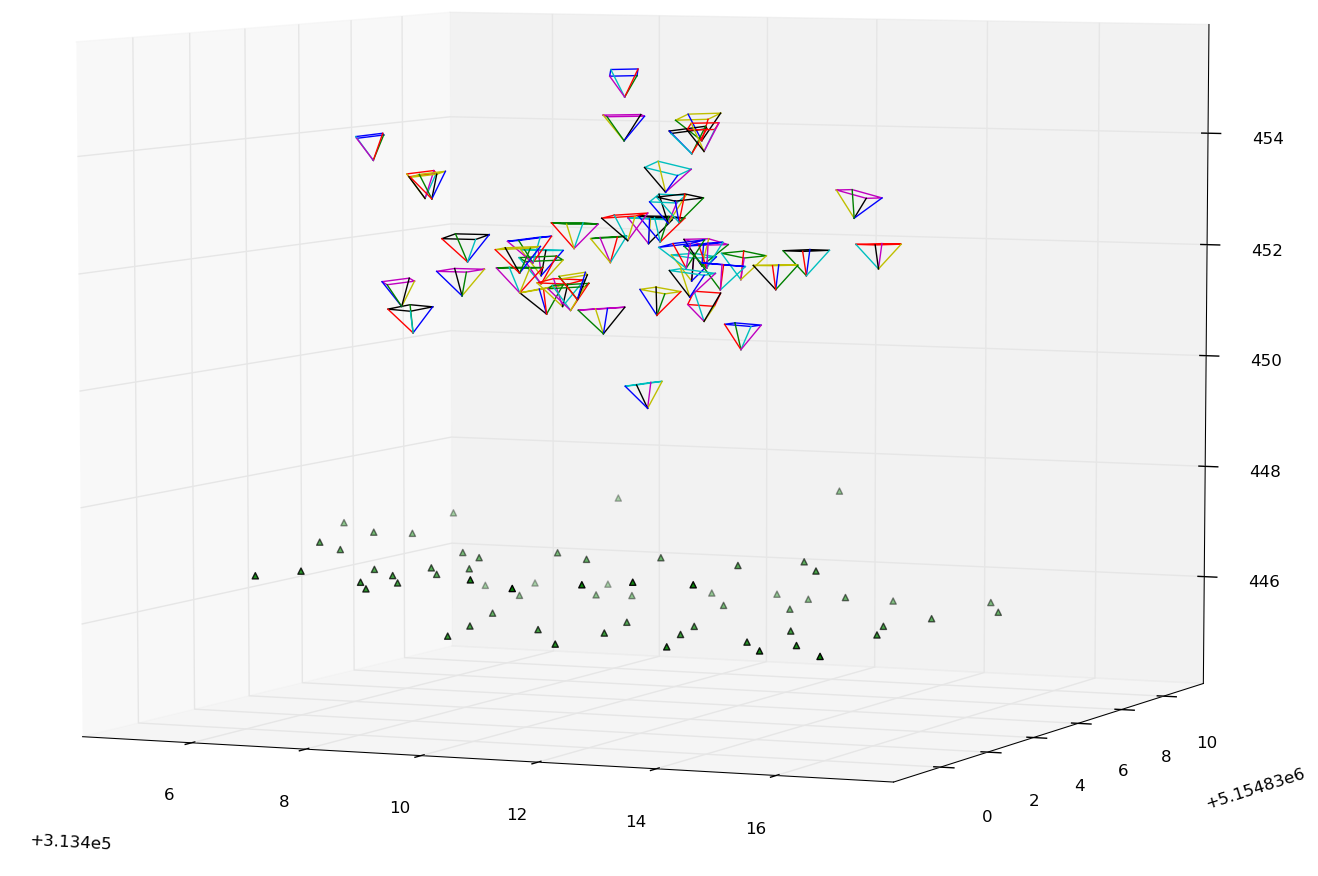
\includegraphics[scale=0.5]{figures/bingo_result.png}
Unlike many other real scenes which can be comprised by hundreds of photos and thousands of tie points,   
there are just a few tie points (64) and photos (45) taken by same camera. Also the photos capture same points thus there 
is lot of redundancy. Solving the scene with such redundant scene should improve robustness of the BBA iteration. 

In the rest of the chapter there will be presented results of subsequent steps, which are performed in processing chain and compared 
to the Bingo-F results.

The first step is relative orientation of pairs. The relative orientations of the pairs were done by OpenCV 5 point algorithm.
The algorithm was successful on most of the pairs, however there are some pairs were algorithm does not work well.

Example of the algorithm success can be showed in this plot:
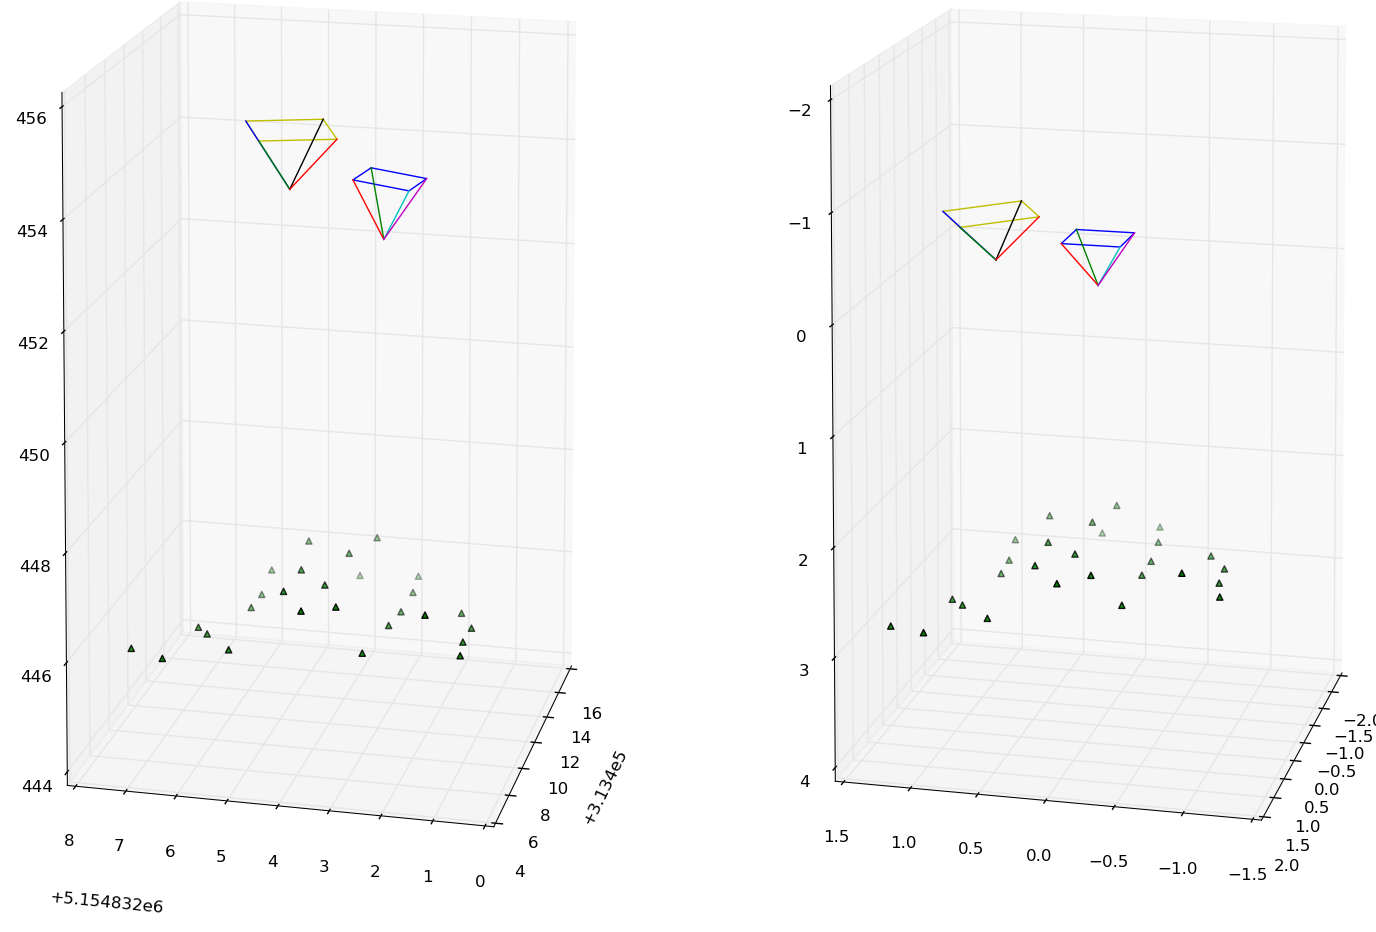
\includegraphics[scale=0.4]{figures/rel_or_576_598.png}
The right plot shows the result of five point algorithm and the left plot shows result of Bingo-F. Note that both 
plots are in different coordinate system, however it is possible to asses it visually. It is clearly visible
that both scenes are very similar.

On the other hand, there exists  few cases, which relative orientation were not successful.  
One of such a cases is relative orientation of photos pair 553 and 591:  
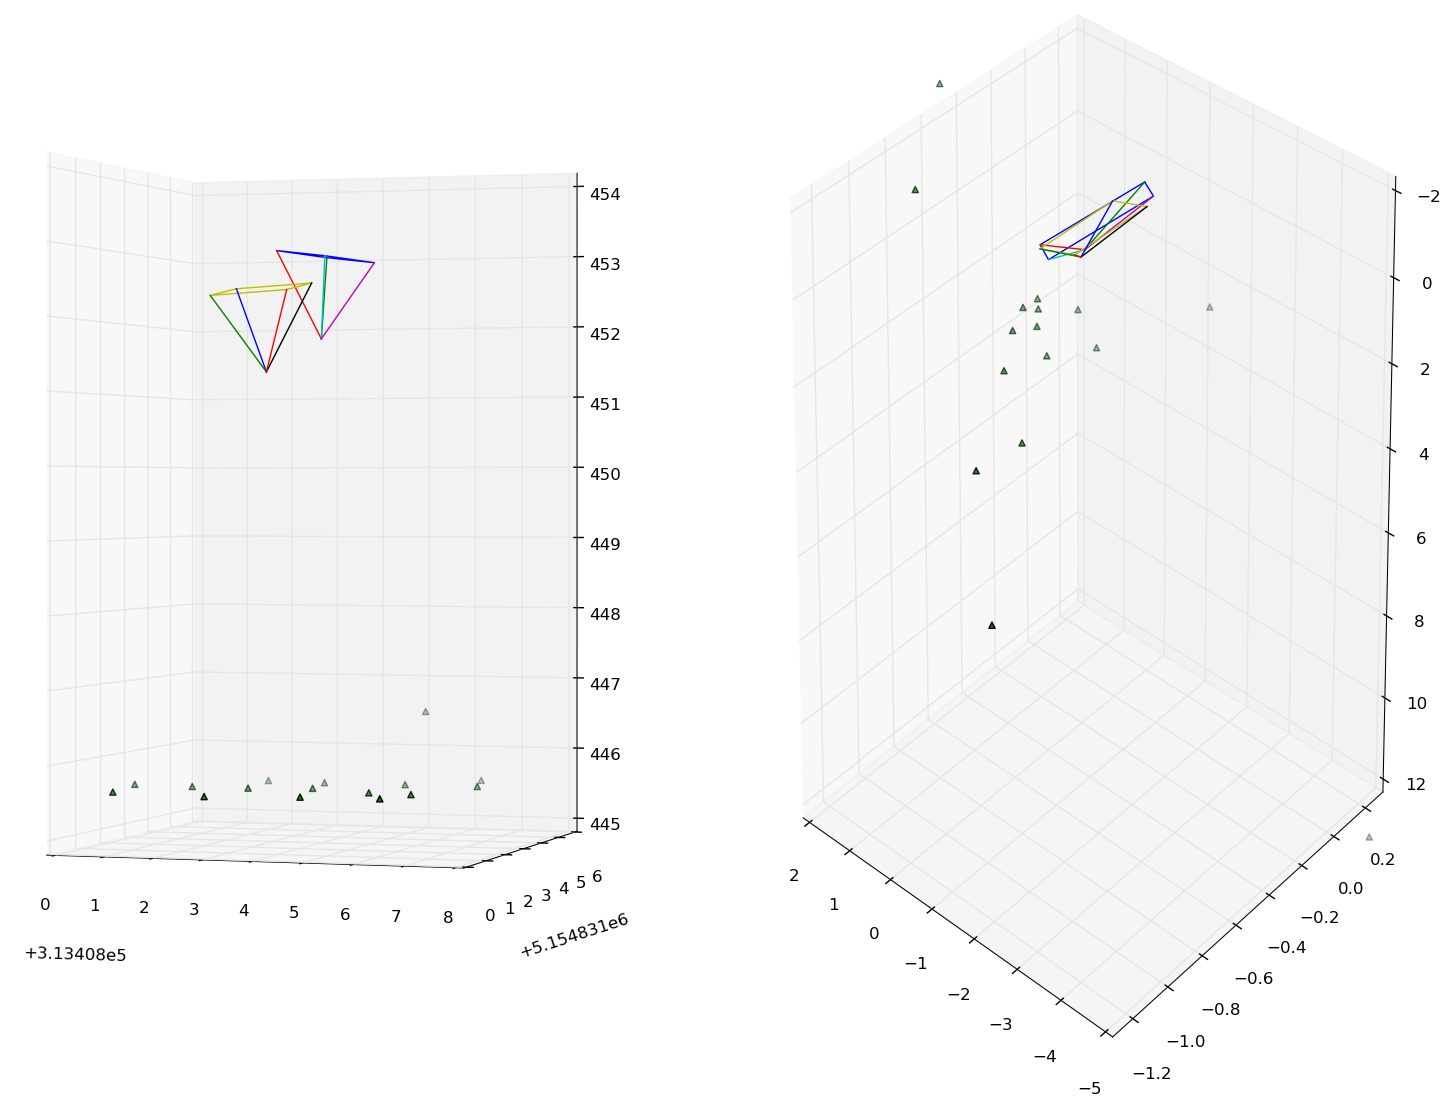
\includegraphics[scale=0.4]{figures/rel_or_553_591.png}
It is clearly visible that result of relative orientation is completely different from the Bingo-F result.
Most important factor, which affects success of the five point algorithm is threshold parameter of RANSAC loop.
The above mentioned relative orientations were computed with RANSAC threshold parameters set to 0.001 mm.
If the threshold parameter is changed in 0.1 mm, the result of relative orientation of pair 553 and 591 improves significantly.
On the other hand another relative orientations go wrong. Therefore with statically set threshold parameter, there are always 
few evidently wrong relative orientations in this scene. Thanks to the configuration of the scene, where lot of photos are 
covering same points, it is  not serious problem, because the point is determined in most relative orientations  with 
much better accuracy, thus it is possible to exclude this outliers. This could be serious problem e. g. if the photos 
of scene would cover long chain where redundancy is much more lower.   
In this case one wrong relative orientation could thread whole result of bba. If error would appear in the middle 
of the chain it would  be propagated up  one half of the chain which transformation on the wrongly
determined pair, which is apparent from equations in \label{eq:comm_rel}. 
In the test case there are not so many critical pairs, which has to be determined correctly to avoid spoiling the transformation 
of the others dependent pairs. Fortunately the reference pair, which defines common relative system, is very stable and also 
the other  core pairs on which depends lot of other pairs are stable. Probably there is some correlation between number 
of points and stability of five point solution, because as it was already mentioned algorithm of merging searches 
for maximum number of tie points from possible relative orientation, thus another way how to improve stability of the solution 
could be identification of another tie points, which could be done automatically by pattern matching algorithms. 
In the test case there 
are 27 tie points in the reference pair. Which gradually decreases to 6 point in the pair, which is merged as last.

During the merging process all object points computed from different relative orientations, which represents same point are 
transformed into  the common relative system. Then the approximate coordinates by object points are determined as median
of point coordinates from different relative orientations. Median was chosen because it is more robust to the effect of 
big outliers caused by few wrong relative orientations in the set. If there is more than 50 percent of coordinates 
which are close to the correct value and the rest are big outliers (luckily the test case is the case), median gives reasonable results over average,
which is much more sensitive to the effect of the big outliers. 

The next step is helmert transformation of the common relative orientation system into the world coordinate system using available GCPs. 
The transformed scene can be compared to the results of Bingo-F adjustment. Average difference of exterior orientation 
of camera is approximately around 0.5 meters with highest outlier in meters. The object points coordinates 
are little bit more accurate with average approximately 20 and highest outliers in 3-1 meters. 
Angles differences are shown in this plot, where there are plotted axes of two camera coordinates systems, which represents 
Bingo-F adjustment angles and the  initial angles. 
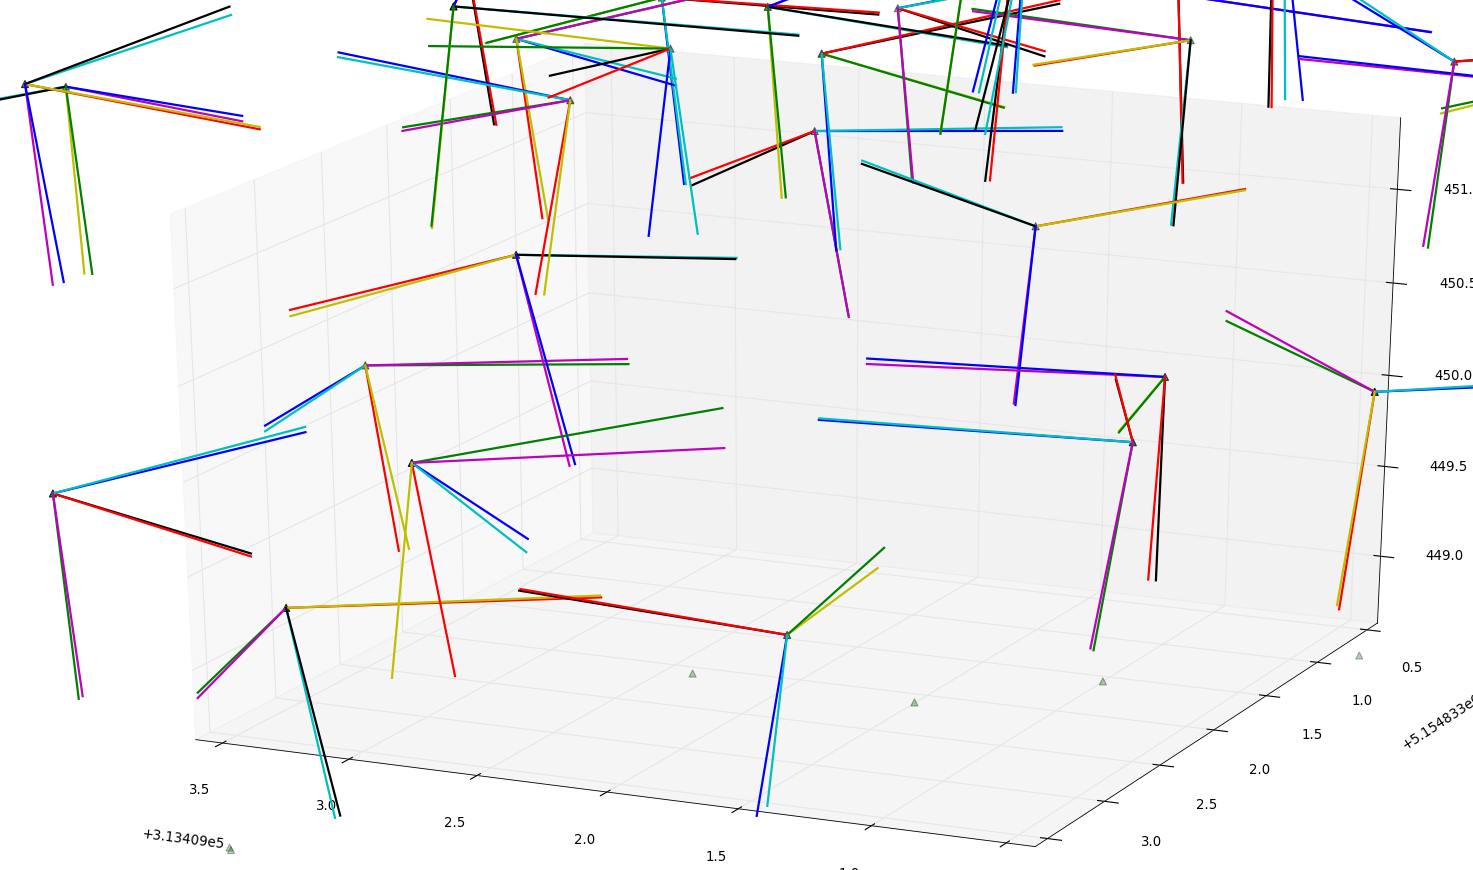
\includegraphics[scale=0.4]{figures/angles_comaprison_relative_orinetaion.png}
It is clear that there are a few orientations, which differs  (tenths of degrees) form the result. 

As a last step bba was applied on these initial values with taking gcp as knowns.
Despite the fact that there were few huge outliers in both parameters of cameras and points,
BBA after five iteration subsequently refines all scene parameter and reduces all cordinates 
differences into the centimeters and angles into the tenths of degrees. 


This plot again shows differences of cameras coordiantes system, which are no longer visible from this point of view
unlike to the previous plot:
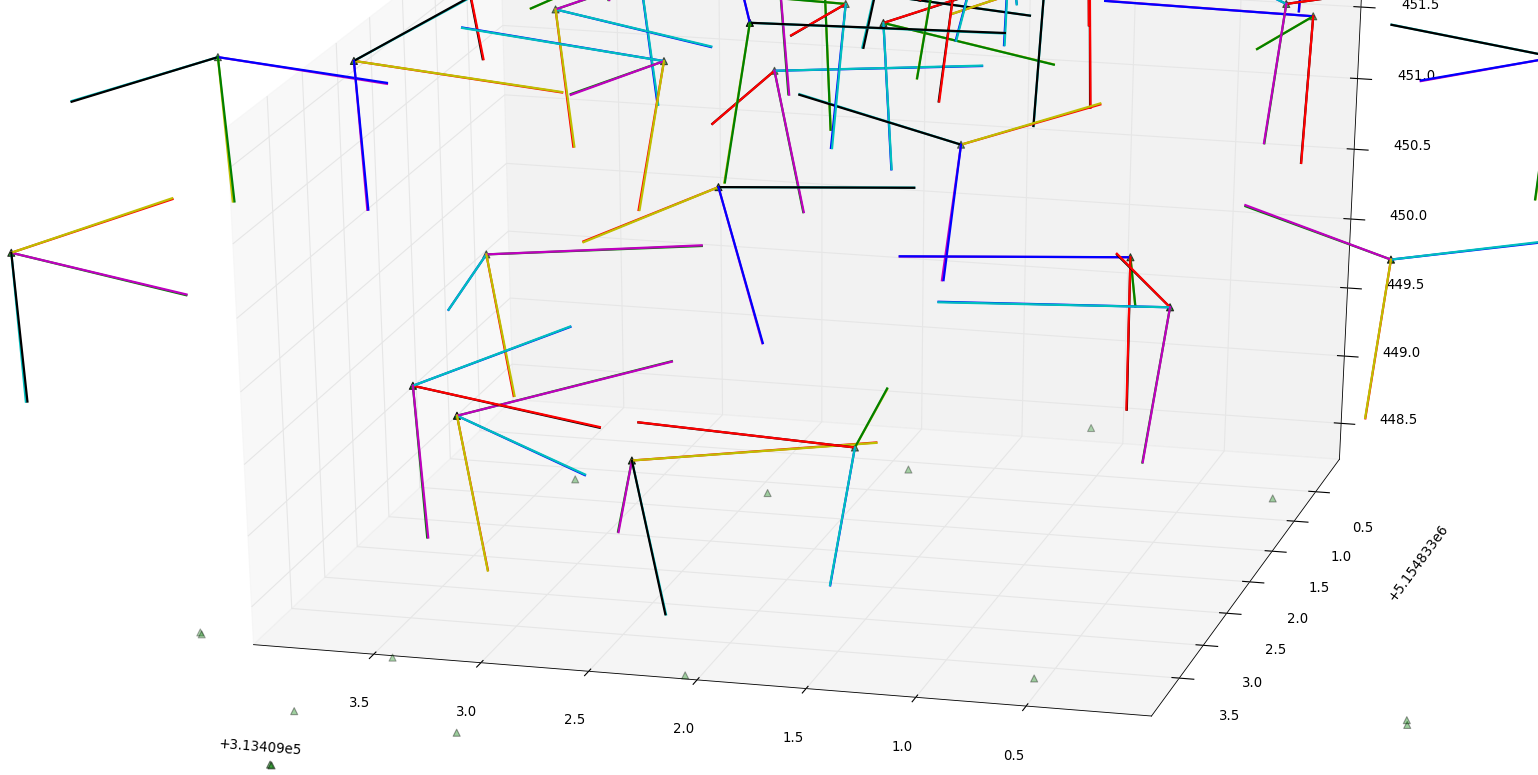
\includegraphics[scale=0.4]{figures/result.png}


\section{Future development}


Basically the work which has been done in this thesis, can be considered as prove of concept,
which shows path of future implementation of BBA in GRASS GIS. The developed 
processing chain in current state cannot be considered as working solution.

Currently  the processing chain was just tested 
 on one scene, where it gives reasonable results. However 
author is sure that in other more complicated scenes it would not work successfully because 
the solution is not robust at all.

In order to improve robustness of the processing chain this suggestions should be considered:
\begin{itemize}
\item Relative orientations - there is no check, whether relative orientation accuracy is successful or not. There 
should be implemented some mechanism, which asses quality of relative orientation (probably according to reprojection error of object points).
Also it should be examined work of the five point algorithm with RANSAC loop on scenes with higher number of the tie points, where 
the outliers elimination effect of RANSAC loop should be much stronger.
\item  Merging of relative orientations - currently if there is one wrong relative orientation, with lot of depended relative orientations,
the error gets propagated up during transformation of depended orientations to the common relative coordinate system. 
Effect of such a inaccurate pair could be 
reduced by performing  temporary BBA, which can fix these some of big inaccuracies. Also the order of relative orientations in merging 
into  should not 
be chosen only by number of tie points but also taking into account quality of relative orientation.

Calculation of scale lacks checks 

\item During final BBA, the weights are ignored using identity matrix. Good choice of weights during every least squares iteration 
could be big leap towards robustness of the BBA. If the weights are selected properly, it is possible to eliminate of outliers 
effect.
Another way how to improve final accuracy of BBA is skipping points, which 
standard deviation from adjustment is higher than some threshold after. The standard deviation criteria can be assessed 
after every iteration.
\end{itemize}


Another big room for improvement is computational speed of the processing chain.
The most critical part which costs most of computational time is BBA.
One least squares  iteration of BBA takes approximately 5 seconds in the test case, which can be 
considered as very small scene compared to commonly the solved
scenes with hundreds of photos and thousands of points. The bottleneck of BBA iteration is computation of inverse/pseudo inverse, where big matrices 
must be solved. The size of the matrix is directly connected to the number of adjusted parameters. There exists  lot of methods which reduce computational 
time of matrix inversion. The inversed matrix of BBA is sparse (most of elements are zeros).

There exists many optimization methods exploiting this property. 
It is also possible to speed up some parts of the code reimplementing them in C instead of currently used Python. However this should be done 
as last step when the part, which is going to be reimplemented in C is tested and works well. Otherwise it would be waste of time and energy, if reimplemented 
code would not be eventually used. 

Another option should which should  be considered is employing of some free software BBA libraries.
Some of the free BBA libraries are:
\begin{itemize}
\item sba
\item Simple Sparse Bundle Adjustment 
\end{itemize}

Both libraries are highly optimized and they are based on Levenberg–Marquardt algorithm.
On the other hand it would require to add new dependency into GRASS, if such a library would be used. 
There is trend to avoid adding new dependencies into GRASS because it already relies on many software libraries,
which makes installation of GRASS sometimes difficult because of countless combinations of library versions.



There is still needed to define interface between the developed modules and also their inteface. 
This thesis outlines just rough architecture of final solution, because at this early stage of development 
there is no point in dealing with the interface, because it can change lot of time during further development.


\section{Conclusion}

\section{References}
%\nobibliography{BP}
\bibliographystyle{plain}
\bibentry{Hartley2004}

\bibentry{wiki:SIFT}

\bibentry{wiki:SURF}

\bibentry{leutenegger2011brisk}

\bibentry{barazzetti2010extraction}

\bibentry{wiki:Eight-point_algorithm}

\bibentry{stewenius2006recent}

\bibentry{bruckner2008experimental}

\bibentry{nister2004efficient}
TODO
\bibentry{pietzsch2001robot}
TODO
\bibentry{pietzsch2004application}

\bibentry{rocchini2012robust}

\bibentry{i.ortho.photo}

\bibentry{neteler2008open}

\bibentry{camera_calibration2013opencv}

\bibentry{zhang2000flexible}

\bibentry{calib_manual2013opencv}

\bibentry{v.rectify}

\bibentry{brown1966distortion}

\bibentry{bingo2013gip}

\bibentry{labe2004geometric}

\section{Appendix}
\subsection{Adjustment protocol}
\label{sec:adj_protocol}


\end{document}}
